\documentclass{article}
\usepackage[utf8]{inputenc}
\usepackage[french]{babel}
\usepackage{graphicx}
\usepackage{listings}
\usepackage{parskip}

\lstset{rangeprefix=\#\ ,% curly left brace plus space
                                 rangesuffix=\ \#}% space plus curly right brace


\title{Compte rendu projet majeur}
\author{Soren LE MEITOUR, \and Mael MONTILLET}
\date{Octobre 2022}

\begin{document}
    \maketitle
    \tableofcontents
        \section{Concept et histoire du jeu}
	\bigskip
	\subsection{L'univers pokemon}
		Dans l'univers des Pokémon, les animaux du monde réel n'existent pas. Le monde est peuplé de Pokémon, des créatures qui vivent en harmonie avec les humains, 						mais possèdent des aptitudes quasiment impossibles pour des animaux du monde réel.

		Certains dressent les Pokémons pour organiser des combats entre eux et nous vous proposons une émulation de ces combats.
	\subsection{La licence}
		Pokémon est une série de jeux vidéo créée par le Japonais Satoshi Tajiri et éditée par Nintendo, selon les statistiques de Nintendo en 2010, les jeux Pokémon se sont 					vendus à environ 250 millions d’unités
	\subsection{Les creatures pokemon}
		Les Pokémon sont des créatures intelligentes ayant un ou deux types et pouvant maîtriser des capacités. Le but de ces combats est simple : il faut mettre le Pokémon 					adversaire K.O. grâce aux capacités, le Dresseur guide son Pokémon en lui donnant des instructions d'attaque.
		Les Pokémon sont capturables par des Poké Balls qui permettent de transporter le Pokémon plus facilement s'il n'est pas utilisé. Un Dresseur ne peut porter avec lui 					que six Pokémon à la fois. Mais peut choisir ses sixs pokemons parmis les 924 pokemons crées à ce jours. Nous avons bien sur enlevé cette posibilité pour des raison 					pratiques. Dans notre version, les deux adversaires auront donc la même équipe composée de bulbizarre, carapuce, étourmi, pikachu, osselait et salamèche 							(pokemons qui appartiennent réellement à la licence).
		Nous avons simplifié le système de statisitique des pokemons (qui présente normalement deux statistiques d'attaques et deux de defense). Chaque pokemon aura donc:
		\begin{itemize}
			\item Une statistique d'attaque.
			\item Une statistique de defense.
			\item Un nombre de PV
			\item Une vitesse qui determine quel pokemon attaque en premier (outre la priorite des attaques et des changements).
			\item Quatre attaques qui infligent un nombre de dégât donné (et qui peuvent avoir des effets autre que les dêgat comme ajouter des statuts, changer de 							pokemon...) et possèdent un type.
			\item Les points de pouvoir ou PP de ses attaques. C'est une liste d'entiers qui represente le nombre de fois que l'attaque i (i l'indice dans la liste) peut être utilisée. Chacun de ces entiers est décrémenté quand l'attaque correspondente est utilisée. Quand les PP sont à 0, l'attaque correspondante n'aura pas d'effet si elle est choisie. Si un pokemon n'a plus de PP sur toutes ses attaques et qu'il reste sur le terrain, il perd 50 PV. Cette statistique est utile pour limiter la taille des parties et s'assurer que les agents ne rentrent pas dans une boucle.
		\end{itemize}

    
\section{Règles du jeu}
	Lors d'un affrontement, chaque dresseur envoie au combat un pokémon. À chaque tour, chaque pokémon utilise une capacité choisie ou est remplacé par un autre pokémon 				de l'equipe. Les choix des actions sont simultanés entre les deux joueurs et l'ordre des événements est regit par plusieurs règles : Les changements sont prioritaires donc effectués 			au debut du tour. Les attaques prioritaires comme vive-attaque passent avant les autres quelque soit la vitesse de leur lanceur. Lorsque deux attaque ont la même priorite, c'est le 			pokemon le plus rapide qui attaque en premier.
	
	Lorsqu'un pokemon est mit K.O., il ne peut pas effectuer d'attaque et un remplacant est choisit par le dresseur concerné.
	
	A la fin de chanque tour, les statuts des pokemons sur le terrain sont appliqués. Quand deux pokemons ont des statuts c'est le pokemon le plus lent qui subit les statuts en premier (c'est important car il peut y avoir la situation où les deux pokemons vont mourir des status et sont les derniers pokemons de l'équipe, le premier qui subit les statut est donc celui qui perd la partie).
	
	Un joueur a perdu quand tout ces pokemons sont K.O..*
        \subsection{Déroulé d'une partie}
        Une fois l'interface, les types et les pseudos des joueurs choisit, la partie débute. Tout d'abord, les deux joueurs choisissent leur pokemon de depart parmis les 6 pokemons disponibles dans notre jeu (se référer au point 3.1 pour plus dinformation). Celui-ci est alors sur le terrain, c'est lui qui combattra en premier. 
        Comme expliqués ci-dessus, à chaque début de tour, les deux joueurs choisiront chacun leur tour entre attaquer le pokemon adverse et échanger le pokemon sur le terrain avec un de ses pokemon disponible, en pouvant jeter un oeil aux informations de la partie pour prendre sa décision. 
        Une fois que les deux joueurs ont éffectuer leur choix, ceux-ci s'appliqueront et le tour sera fini.
        Tant qu'un des deux joueur n'a pas perdu tout ses pokemons, les tours se succederont de cette façon.


 
	\subsection{Calcul des dégât d'une capacite}
		Si on note a l'attaque du pokemon attaquant, la d la defense du pokemon defenseur et c les dégâts de l'attaque, la formule pour calculer les degâts (dans notre version 					simplifiée) est  :
		\[
			\frac{a}{d} * c
		\]
		Avec un bonus de 10\% si le type de l'attaque est le même que celui du pokemon qui la lance.
\section{Notre version du jeu}
	\subsection{Les pokemons disponibles dans notre jeu}
		\subsubsection{Boulbizarre}
            \begin{center}
				
\includegraphics[width=4cm,height=4cm]{images/boulbizarre}
			\end{center}
			\begin{itemize}
				\item Type : plante
				\item Attaque : 120
				\item Defense : 120
				\item PV : 230
				\item Vitesse : 110
				\item Listes des attaques : Fouet-Liane (de type plante, inflige 90 de dégât), Charge (de type normal, inflige 60 de dégât), Croissance (de type normal, inflige 0 dégâts et multiplie le bonus d'attaque 'a'[voir 2.1] par 1,25) et Vampigraine ( de type plante, applique le statut vampigraine)
			\end{itemize}
			Remarque stratégique : L'attaque Vampigraine de bulbizarre est très utile sur le long terme grâce à son pourvoir de soin. Ce pokemon est un très bon tank avec son grand nombre de PV, capable d'encaisser les attaques tout en mettant des bons dégâts. Il est cependant un peu lent.
		\subsubsection{Carapuce}
            \begin{center}
				
\includegraphics[width=4cm,height=4cm]{images/carapuce}
			\end{center}
			\begin{itemize}
				\item Type : eau
				\item Attaque : 120
				\item Defense : 150
				\item PV : 230
				\item Vitesse : 110
				\item Listes des attaques : Exuviation (de type eau, inflige 0 dégâts et multiplie les bonus d'attaque et de defense 'a' et 'd' [voir 2.1] respectivement par 1,5 et 0,75), Ebullition (de type eau, inflige 80 de dégât et le statut brulure avec une chance sur trois), Toxic (de type normal, inflige 0 dégâts et applique le statut poison) et Coud-Boule (de type normal, inflige 75 de dégât)
			\end{itemize}
			Remarque stratégique : Carapuce est un pokemon avec une grosse defense et qui a la possibilité d'appliquer plusieurs statuts. Il est donc tres intéressant lorsqu'il s'agit de se placer, notamment grâce à son attaque éxuviation qui permet d'augmenter beaucoup son attaque, bien qu'en prenant le risque de baisser sa defense
		\subsubsection{Etourmi}
            \begin{center}
				\includegraphics[width=4cm,height=4cm]{images/étourmi}
			\end{center}
			\begin{itemize}
				\item Type : vol
				\item Attaque : 130
				\item Defense : 90
				\item PV : 220
				\item Vitesse : 110
				\item Listes des attaques : Vive-attaque (de type normal, inflige 70 de dégât), Atterrissage (de type vol, inflige 0 dégâts et soigne étourmi à hauteur de la moitié de ses PV de base), Rapace (de type vol, inflige 100 de dégât) et Antibrume (de type vol, inflige 0 dégâts, retire le statut piège de rock si celui-ci est présent)
			\end{itemize}
			Remarque stratégique : Malgrès son faible potentiel defensif, étourmi compense par une possibilité de soin et surtout par de gros dégâts et la possibilité de s'assurer d'attaquer en premier avec vive-attaque, très utile pour finir un pokemon avant qu'il soit changer par exemple.
		\subsubsection{Pikachou}
            \begin{center}
				
\includegraphics[width=4cm,height=4cm]{images/pikachou}
			\end{center}
			\begin{itemize}
				\item Type : electrik
				\item Attaque : 130
				\item Defense : 110
				\item PV : 210
				\item Vitesse : 200
				\item Listes des attaques : Tonerre (de type electrik, inflige 95 de dégât), Cage éclair (de type electrik, inflige 0 dégâts et applique le statut Paralysé si l'adversaire n'est pas de type electrik), Rugissement (de type normal, inflige 0 dégâts et multiplie le bonus d'attaque 'a'[voir 2.1] de l'adversaire par 0,75) et Change-éclair (de type electrik, inflige 70 de dégât et permet de changer de pokemon tout de suite après l'attaque)
			\end{itemize}
			Remarque stratégique : Pikachou est idéal pour faire mal rapidement. En effet, il a une bonne attaque et une vitesse qui lui assure, sauf cas particulier, de toujours attaquer en premier. Son attaque change-éclair permet, au lieu de simplement changer de pokemon, d'infliger des bons dégâts avant de le faire.
		\subsubsection{Osselait}
            \begin{center}
				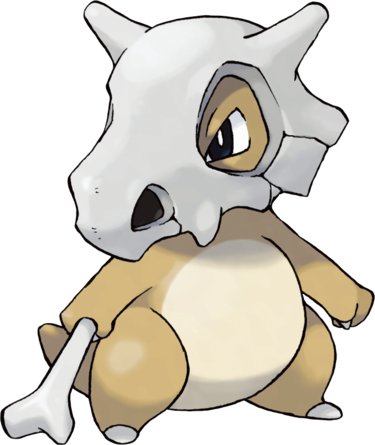
\includegraphics[width=4cm,height=4cm]{images/osselait}
			\end{center}
			\begin{itemize}
				\item Type : sol
				\item Attaque : 120
				\item Defense : 200
				\item PV : 240
				\item Vitesse : 95
				\item Listes des attaques : Mimi-queue (de type normal, inflige 0 dégâts et multiplie le bonus de defense 'd' [voir 2.1] de l'adversaire par 0,75), Seisme (de type sol, inflige 100 de dégât), Piège de rock (de type sol, inflige 0 dégâts et applique le statut piège de rock) et Coud-Boule (de type normal, inflige 75 de dégât)
			\end{itemize}
			Remarque stratégique : Meilleur defenseur du jeu, osselait peut resister très longtemps à ses adversaires. Son attaque seisme fait d'énorme dégâts et son attaque piège de rock permet de blesser les pokemons adverses progressivement, à chaue changement de pokemon adverses.
		\subsubsection{Salamèche}
			\begin{center}
				
\includegraphics[width=4cm,height=4cm]{images/salameche}
			\end{center}
			\begin{itemize}
				\item Type : feu
				\item Attaque : 130
				\item Defense : 110
				\item PV : 220
				\item Vitesse : 150
				\item Listes des attaques : Crocs feu (de type feu, inflige 65 de dégât et le statut brulure avec une chance sur trois), danse flammes (de type feu, inflige 35 de dégât et le statut emprisonne), tranche (de type normal, inflige 70 de dégât) et groz yeux (de type normal, inflige 0 dégâts et multiplie le bonus de defense 'd' [voir 2.1] de l'adversaire par 0,75 tout en multipliant son bonus d'attaque 'a' [voir2.1] par 1,25)
			\end{itemize}
			Remarque stratégique : L'attaque danse flammes est utile pour bloquer le pokemon adverse sur le terrain et mettre face à lui un pokemon qui le contre afin de le mettre KO ou de se placer. La vitesse élevée du salamèche lui permet aussi de facilement finir des pokemons affaiblits.
	\subsection{Les statuts disponibles dans notre jeu}
		\subsubsection{Brulure}
			Statut qui inflige des dégâts à hauteur d'un huitième des PV totaux du pokemon à chaques tours pendant 6 tours et multiplie son bonus d'attaque 'a' [voir 2.1] par 2/3,
		\subsubsection{Poison}
            Statut qui inlige des dégâts à hauteur de 1/16, 2/16, 3/16 puis 4/16 des Pv totaux du pokemon, respectivement pendant le 1er, 2ème, 3ème et 4ème tour durant lesquels il s'applique.
		\subsubsection{Vampigraine}
            Le pokemon affecté voit sa vitesse être réduite de moitié et se fait 'vampiriser', Il perd des PV à hauteur de 1/8 de ses PV totaux et le pokemon qui a lancé vampigraine récupère ces PV. Ce statut s'applique pendant 5 tours.
		\subsubsection{Paralysie}
            Le pokemon affecté par ce statut a 1 chance sur 3 de ne pas pouvoir attaquer au tour suivant et voit sa vitesse être réduite de moitié. Ce statut s'applique pendant 10 tours
		\subsubsection{Emprisonnement}
            Le pokemon affecté ne peut pas être échangé avec un autre pokemon pendant 6 tours.
        \subsubsection{Piège de rock}
            Le dresseur étant coincer sous les pierres pendant 30 tours, le pokemon arrivant sur le terrain en cas de changement de pokemon de sa part reçoit directement des dégâts en fonction de son type :
            \begin{itemize}
                \item 18/100 de ses PV totaux si il est en faiblesse par rapport au type sol
                \item 12/100 de ses PV totaux si il n'est ni en faiblesse ni en resistance par rapport au type sol
                \item 6/100 de ses PV totaux si il est en resistance par rapport au type sol
                \item rien si il est immunisé au type sol
            \end{itemize}
    \subsection{Tableau des types disponibles dans notre jeu}
        \begin{center}
			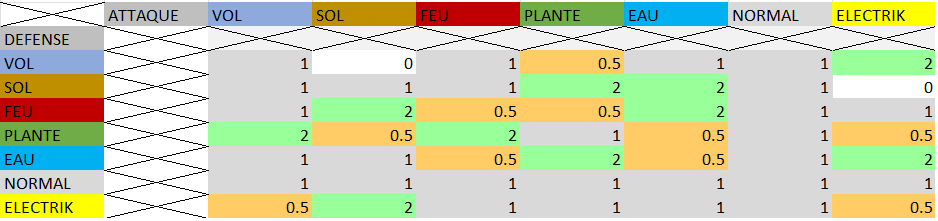
\includegraphics[width=15cm,height=4cm]{images/tableau_type}
		\end{center}
        Voici un tableau presentant les rapports entre les différents types:
        \begin{itemize}
        \item Se lit " le type 1 (colonne) est en faiblesse, resistance, immunité ou normal par rapport au type 2 (ligne) si le coefficient est respectivement 2, 0.5, 0 ou 1
        \end{itemize}
        \bigskip
        \section{Architecture du code}
    Dans cette partie nous allons voir comment nous avons structuré nos programmmes, c'est un point important qui définit les performences, la robustesse et la facilité à s'adapter à de nouvelles situations de l'application produite.
    \subsection{Idée générale}
        Nous avons cherché le plus possible à utiliser les classes dès que c'était necessaire, car la \textebf{programmation orienté objet} permet une meilleure lecture du code et plus de souplesse et de facilité dans son dévelloppement.
        
        Pour la plupart des problèmes nous avons cherché à produire une \textbf{class abstraite} mère qui correspondait à l'idée générale de ce que nous voulions coder et plusieurs classe filles, plus spécifiques qui en héritait. Cette manière de proceder à l'avantage de rendre plus clair le code et de facilité l'ajout de nouvelle fonctionalité. Par exemple pour ajouter un pokemon il suffit de créer une nouvelle classe qui hérite de la classe abstraite Pokemon. 
        
        Ensuite, un autre avantage de l'orienté et de l'héritage des classes abstraites c'est de cloisonner les problèmes. En effet, quand par exemple un jeu discute avec une interface, il lui fait des requêtes (comme lui demander une action, ou appeller une animation) sans se soucier de si c'est une interface texte ou graphique.
        
        Aussi, nous avons utilisé de nombreuses property, soit pour stocker une information d'une manière différente qu'elle est utilisée, soit pour être sûr que des attributs ne sont pas modifiées en dehors de leur classe. Par exemple, pour être sûr que le pokemon courant d'un dresseurs soit un des pokemons de son dictionnaire de pokemon, self.\_\_courant stocke le nom d'un pokemon puis un property fait en sorte que self.courant soit le dictionnaire indexé par le nom stocké dans self.\_\_courant.
        
        Enfin l'orienté objet permet d'utiliser des solutions de code qui sont générales et réutilisables dans d'autres situation. Par exemple, les solution utilisant l'algorithme du minimax sont des solution générales appliquées à notre jeu.
    \subsection{Diagramme UML}
        Voici le diagramme UML de notre jeu, réalisé avec PlantText UML. Etant donné du grand nombre de classes présentent dans notre jeu, nous avons décidé de limiter le diagramme UML aux classes principales en représentant leurs classes dérivées par une seule classe Exemple. Par exemple, notre jeu comporte une classe abstraite Attaque, qui se dérive en 23 sous-classes pour les 23 différentes attaques présentent dans notre jeu. Celles-ci sont représentées dans le diagramme par la classe Exemple\_attaque.

        Dans ce diagramme, les attributs et les méthodes sont représentés respectivemement dans les parties hautes et basses des classes. Voici une légende pour mieux comprendre les signes qui peuvent apparaître devant ceux-ci.
        \bigskip
        \begin{itemize}
            \item Une classe portant la mention 'C' à côté de son nom est une classe normale
            \item Une classe portant la mention 'A' à côté de son nom, qui est écrit en italique dans ce cas, est une classe abstraite.
            \item Un rond vert non plein représente un attribut publique d'instance.
            \item Un carré rouge non plein représente un attribut privé d'instance.
            \item L'absence de signe représente un attribut de classe.
            \item Un rond vert plein représente une méthode basique.
            \item Un carré rouge plein une méthode avec une property.
            \item Une méthode soulignées représente une méthode statique.
            \item Une méthode en italique représente une méthode abstraite.

            
        
        \end{itemize}
        Remarque : pour mieux voir le diagramme, veuillez regarder directement le png(images/Diagramme\_UML)
    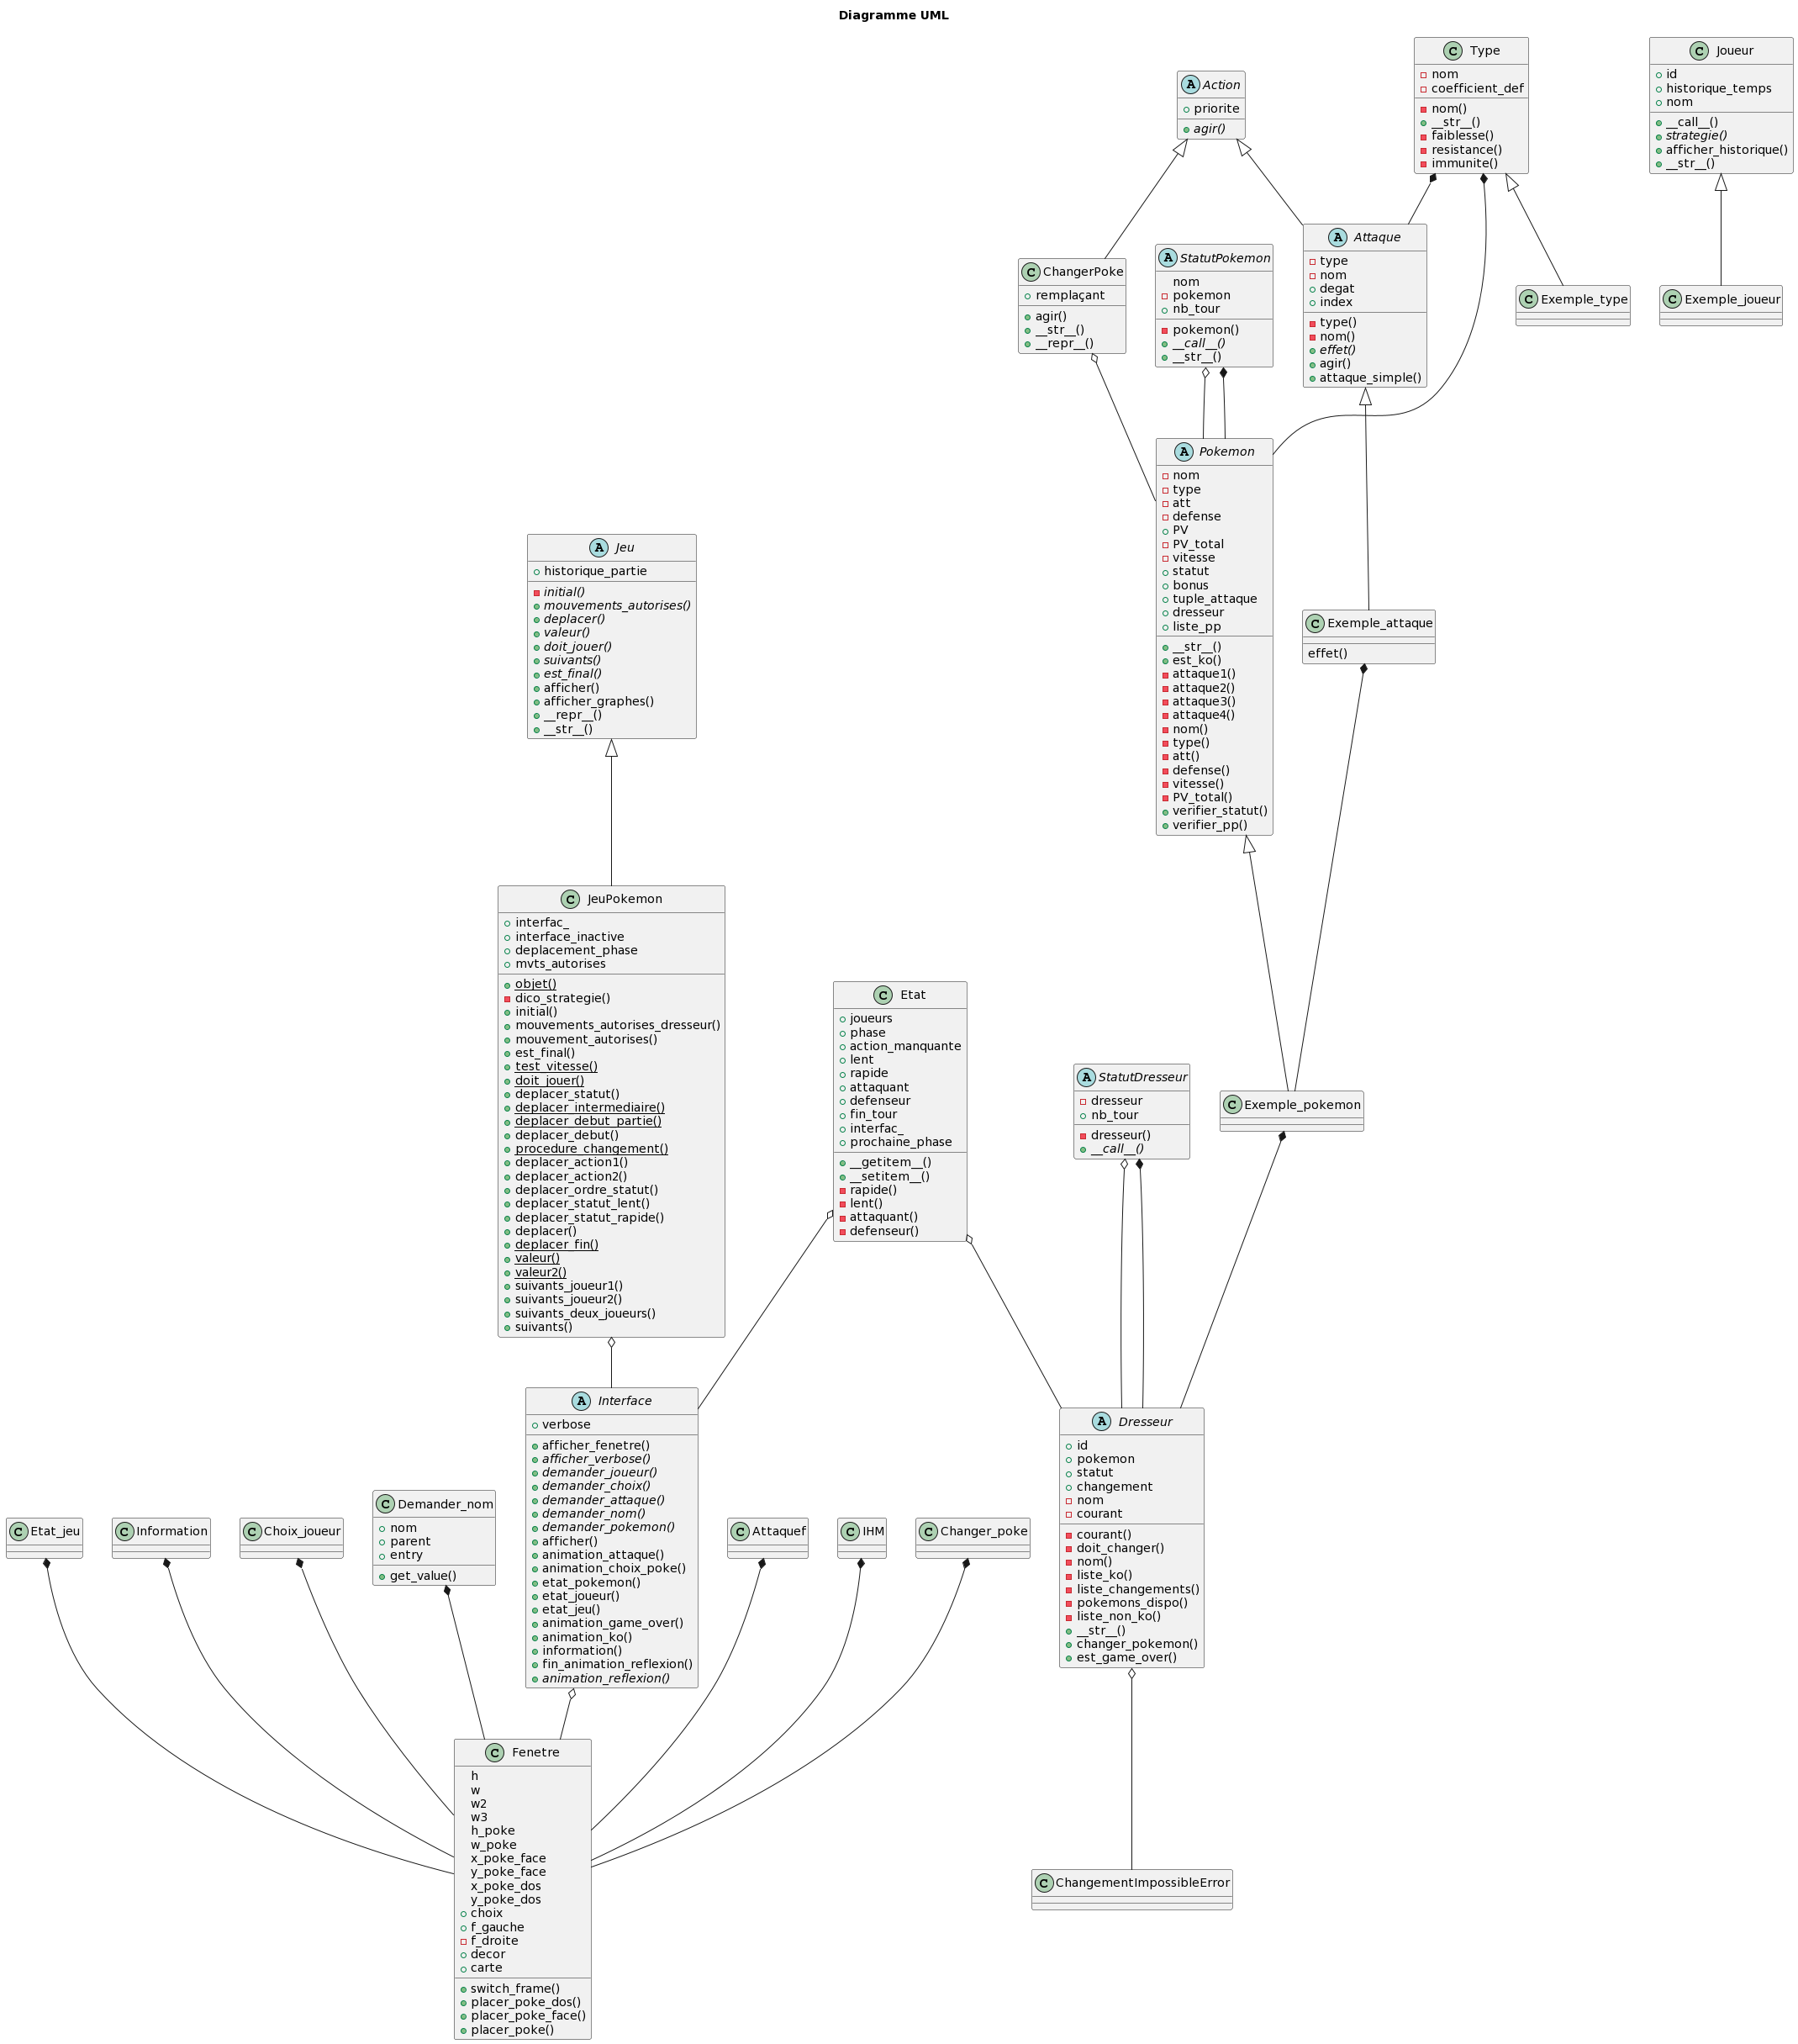
\includegraphics[width=20cm,height=20cm]{images/Diagramme_UML}
        
    \subsection{Architecture du jeu}
        Afin de pouvoir appliquer des solutions générales comme l'algorithme du minimax à notre jeu, il fallait que notre jeu soit une classe JeuPokemon qui hérite de la classe Jeu présentée dans le cours et qu'il soit lancé via joueur\_jeu.
        Pour ce qui est de la classe mère, elle a été reprise tel quel dans notre code, cependent la fonction jouer\_jeu était plus problèmatique.
        
        En effet la fonction jouer\_jeu qui nous a été présenté en cours s'appliquait a un jeu :
        \begin{itemize}
            \item à somme nulle (les interêts des joueurs sont strictement opposés).
            \item deterministe (pas d'intervention de la chance).
            \item sequentiel (l'ordre des déscisions et prédéfinit à l'avance)
            \item à information complètes (on connait ses possibilités d'action, les possibilités d'action des autres joueurs, les gains résultants de ces actions et les motivations des autres joueurs).
        \end{itemize}
        Cependent le jeu pokemon que nous vous proposons est à somme nulle, \textbf{non deterministe}, \textbf{simultané} (les joueurs décident en même temps de leur stratégie) et à information complètes.
        Nous avons donc modifié jouer jeu pour qu'elle s'applique à tout les jeux qui ont ces dernières propriétés.
        
        Aussi, nous avons transormé le while qui était dans la fonction en récursivité pour pouvoir animer le jeu avec la méthode after de tkinter mais cette modification ne change rien à ce que fait la fonction.
        Comme nous allons y faire référence dans les prochaines sections, voici la fonction joueur\_jeu:
        
        \lstinputlisting[language=Python, tabsize=1,basicstyle=\scriptsize , linerange=jouer\_jeu-end,includerangemarker=false]{code/abstract_jeu.py}
        
        \subsubsection{Jeu simultané}
            Un jeu simultané est un jeu dans lequel l'ordre de prise de déscision n'est pas prédéfinit. Selon les situation, un joueur doit prendre une descision, l'autre ou les deux en même temps. Une fois les déscision prises, un système de priorité des action permet de definir quelle action est executée en premier ou si même l'action est executée.
            Ainsi, la mèthode doit\_joueur d'un tel jeu ne renvoie pas le joueur qui jou dans un etats mais la liste des joueur qui doivent joueur.
            
            Ensuite joueur\_jeu doit demander la stratégie adoptée par chaque joueur qui doit jouer et la stocker dans deplacements qui est donc un dictionnaire qui prend comme clefs les joueurs et comme valeur les action des joueurs.
            Deplacement est ensuite fournit à deplacer pour deplacer l'etat.
        \subsubsection{Jeu non deterministe}
            Pour pouvoir prendre en compte le facteur chance, deplacer doit revoyer non pas un etat mais l'ensemble des couples des etats possibles avec leur probabilité d'apparition.
            
            Ensuite la fonction choix est utilisée pour choisir un état parmit ceux qui sont possibles.
            \lstinputlisting[language=Python, tabsize=1,basicstyle=\scriptsize , linerange=choix-end,includerangemarker=false]{code/choix.py}
        \subsubsection{Le cas particulier de pokemon}
            Pour que la classe JeuPokemon puisse respecter ce qui a été dit ci-dessus, cela a été un vrai défit de programmation.
            
            Tout d'abord un premier challenge a été de faire en sorte que la fonction deplacer s'arrête à chaque fois qu'il faut demender un choix a un des joueurs, et reprendre ensuite là où elle en était.
            Dans pokemon, un choix est demandé à chaque début de tours aux deux joueurs, puis à chaque fois qu'un pokemon est mit ko au dresseur à qui appartient le pokemon.
            \smallskip
            Ainsi, nous avons découpé le jeu en plusieurs phases, stockées dans l'etat, qui se suivent et représentent des blocs entiers sans choix posés aux joueurs. A chaque phase correspond une fonction de deplacement.
            
            De ce fait, la fonction déplacer correspond à une boucle while dans laquelle on effectue la fonction de deplacement de la phase tant que l'etat ne nous indique pas que le tour est finit.
            
            Les blocs sont les suivants :
            \begin{itemize}
                \item "debut de partie" : en tout debut de la partie, quand les dresseurs n'ont pas de poemon courant et qu'on ne peut pas faire de test de vitesse.
                \item "debut" : en debut de tour, permet de definir qui attaque en premier.
                \item "action1" : on effectue l'action du joueur qui joue en premier. 
                \item "action2" : on effectue l'action du joueur qui joue en second
                \item "ordre statut" : Si les deux joueurs ont des statuts, on definit l'ordre dans lequel ils les subiront. Si il n'y en a qu'un on les effectue directement (car pas besoin de differencier le lent et le rapide).
                \item "statut lent" : On effectue les effets de statuts du pokemon le plus lent.
                \item "statut rapide" : On efffectue les statut du joueur le plus rapide.
                \item "fin" : on verifie si on doit enlever des statuts des pokemons.
            \end{itemize}
            \paragraph{Solution au problème des interruption dans le tour :}
                A chaque fin de bloc, la phase de l'etat est mise soit à la prochaine phase soit à une phase intermédière quand un pokemon à été mit KO. L'ordre du déroulé n'est bien sur pas linéaire et ne suit pas la liste précedente. Par exemple si aucun des joueurs n'a de statut, on passe directement de "ordre statut" à "debut".
                
                Quand la phase est mise à intermédiaire, on stocke dans l'etat la prochaine phase et on signale au while que c'est la fin du tour. Ensuite le pokemon de remplacement est demandé au joueur qui a un pokemon ko et la partie reprend par le deplacement de la phase intermediaire qui effectue le changement demandé par le joueur. Puis la phase prend pour valeur la phase qui avait été stockée dans l'etat comme étant la prochaine phase et le deroulé de la partie reprend.
                
                Bien sûr, la phase qui est stockée avant une phase intermediaire comme étant la prochaine phase depend des événements dans la partie. Par exemple lors du deplacement de "action1", si c'est le joueur qui a fait l'action qui est mit KO en la faisant (par exemple si un pokemon qui a peu de PV est placé en remplacement sur des pièges de rock, il peut être mit KO), alors la prochaine phase sera "action2". Cependent si c'est le joueur qui attaque en second qui est mit KO pendent "action2", alors, la prochaine phase sera "ordre statut" car un pokemon qui est mit KO ne peut pas attaquer dans le tour.
                
                Enfin pour que la partie puisse reprendre correctement après une interruption, on est parfois amené à stocker dans l'etat des information comme l'attaque du second attaquant ou le pokemon qui doit subir les statuts lent... Ce stokage est fait dans l'etat qui est donc une instence de la classe Etat. La classe Etat possède de nombreux attributs dont ces informations intermediaires, la phase, les dresseurs... (voir abstract\_jeu.py)
            \smallskip
            \paragraph{Deplacement de tout les Etats possibles :}
                Le déroulé présenté dans le paragraphe précédent correspond à la fonction deplacer telle qu'elle était avant qu'on ne prenne en compte l'aléatoire.
                
                Ainsi deux changement majeur on été fait pour prendre en compte les branches liées à la chance : 
                \begin{itemize}
                    \item Toutes les action renvoient des couples d'etat possibles avec la probabilité associée, ainsi, toute les fonctions de deplacement renvoient elles aussi le même type de couple.
                \end{itemize} La fonction deplacer travaille avec des listes qui stockent tout les etats possible qui ne sont pas encore finit, et a chaque tour du while, elle parcours la liste pour deplacer la phase suivante de tout ces etats.  A chaque fois qu'un etat est déplacé, ce qui est récupéré est une liste d'etats possible liés au deplacement de cet etat particulier, la probabilite de tout les etats de cette liste est donc multipliée par la probabilite de l'etat dont ils sont issus.
                
                A chaque fois qu'un etat est finit, il est stocké avec sa probabilité dans la liste finale, sinon il est stoké avec sa probabilité dans une liste des etats qui restent à deplacer. La boucle while s'arrête quand il ne reste plus d'etats possibles qui ne sont pas finits.
                
        \subsubsection{Les fonctions suivants}
            Pour les jeu simultanés il y a une petite subtilité par rapport aux etats suivant, c'est que si l'autre joueur doit joueur dans l'etat suivant, il faut présicer quelle action il fait pour réelement, c'est ce qui a été fait dans notre jeu. Ainsi, il ya a deux fonction suivant qui ont principalement été utilisée : suivants\_joueur1 et suivants\_joueur2. On leur fournit deux informations : l'etat et si l'autre joueur joue avec dans ce cas là, son action. La fonction renvoie l'ensemble des triplet action du joueur 1, action du joueur 2, liste des etats possibles avec leur probabilité, sachant que les action de l'autre joueur seront donc soit toutes les même si il joue soit None si il ne joue pas
            
            Voici le code :
            
            \lstinputlisting[language=Python, tabsize=1,basicstyle=\scriptsize , linerange=suivant-end,includerangemarker=false]{code/jeu.py}
        \bigskip
        \section{Strategies}
    \bigskip
	\subsection{Presentation du problème}
		\subsubsection{L'objectif}
			Dans cette partie, nous allons analyser les stratégies envisageables pour jouer à Pokemon. Notre objetif sera de créer une IA capable de jouer à pokemon de la 						manière la plus performante possible sans que le temps de calcul ne soit trop grand.

			Pour cela nous envisagerons d'abord des solutions simples qui s'appuient sur l'aléatoire et sur des règles simples, puis nous travaillerons sur des IA plus performantes 					qui reposent sur les algorithmes généraux présentés en cours et enfin nous essayerons d'améliorer ces algorithmes pour qu'ils s'adaptent mieux à notre jeu.
		\subsubsection{Difficultés liées au jeu pokemon}
			Dans le papier de recherchce \textbf{Learning complex games through self play - Pokémon battles} de \emph{Miquel Llobet Sanchez}, l'auteur cherche à créer une IA 					qui joue à pokemon via des algorithmes de parcours de graphe utilisant du deeplearning (solution qui est généralement celle utilisée pour le jeu pokemon).

			Ce jeu y est présenté comme un jeu qui représente un challenge pour les intelligences artificielles (même modernes) pour les raisons suivantes:
			\paragraph{L'atomicité des tours :}
				A chaque tour, les deux joueurs soumettent une action, et la résolution des actions se fait en même temps via un systeme de priorité des actions (voir règles 						du jeu). Il en résulte que le jeu ne peut pas réellement être représenté comme un arbre et que le plus souvent, les joueurs éxecutent leurs actions dans des états 							différents de celui dans lequel l'action à été choisie.
			\paragraph{Le coût de simulation :}
				Il faut 5 à 40 ms aux moteurs de simulation de bataille pokemons opens sources pour simuler un tour. Sachant que notre version sera vraisemblablement moins 							optimisée, le coût de simulation sera un facteur trés limitant dans le nombre d'états qui pourront être explorés par nos agents.
			\paragraph{Stochasticité :}
				Le jeu pokemon n'est pas un jeu déterministe, la chance influence fortement l'issue des tours. Elle intervient dans le système de priorité : deux pokemons qui 				ont la 	même vitesse auront une chance sur deux d'attaquer en premier si les attaques ont la même priorité (sachant que dans notre version, seule vive-attaque 
				a une priorité differente). Certaines attaques incorporent des facteurs chances comme Ebullition qui possède une chance sur trois de brûler l'adversaire, et les 							statuts aussi (exemple : un pokemon paralysé a une chance sur trois de ne pas attaquer). Un agent qui saura prendre en compte le facteur chance aura donc un 					avantage certain sur les autres agents.
			\paragraph{Le facteur de branchement :}
			 	Sans prendre en compte la Stochasticité, le facteur de branchement est de 4 à 9 (4 attaques et 5 changements potentiels).  Ce n'est pas comparable au facteur de 						branchement des échecs qui est en général autour de 35-38 mais cela reste non négligeable. D'autant plus que le facteur chance peut multiplier le nombre de 						branches par un coefficient compris entre 2 et 4 (ou plus dans de rares cas).
			\paragraph{Difficulté d'apréciation des etats}
					Certaines attaques comme piège de rock (pose des pièges qui inflige des dégâts à chaque changement de pokemon de l'adversaire) ont un effet sur le long 							terme qui sera difficile à apprecier pour les agents car ceux-ci seront forcement limités en terme de profondeur.
					De plus, les pokemons peuvent avoir un certain nombre de statut en même temps et de bonus qui vont être difficiles à apprécier.
    \subsection{Evaluation de l'état}
		Une fonction d'évaluation de l'état de bonne qualité est nécessaire pour créer des agents performants pour deux raisons principales. D'abord, c'est un outil trés intérressant 				pour évaluer les performances d'un agent. On pourra tracer le graphe de la fonction d'évaluation en fonction du nombre de tour lors d'un combat entre deux agents pour 					évaluer leurs performances tout au long de la partie. Ensuite, la fonction d'évaluation est necessaire à certains agents (ceux qui utilisent le minimax) pour avoir une 						approximation de l'utilité (les parties faisant en général plus de 30 tours, il est irréalisable de simuler la partie jusqu'à la fin pour ces agents).

		La fonction d'évaluation doit être rapide à calculer et representer le mieux possible l'état de la partie. Nous avons donc choisi de prendre la difference des PV de tout les 					pokemon du joueur 1 et de tout les pokemon du joueur 2.
		Le joueur max sera donc toujours le joueur 1 et le min le joueur 2 L'avantage c'est que cette fonction est rapide de calcul et 				représente bien ce qui est la clef de la victoire, les PV des pokemons.
		Le défault c'est quelle ne prend pas en compte les types des pokemon , leurs bonus et statuts, et leurs statistiques. Cependant tout ces éléments rajoutent du temps de 					calcul et demandent une connaissance du jeu que nous n'avons pas. Nous avons donc décidé de ne pas les prendre en compte.
		La prochaine étape pour améliorer nos agent serait d'entrainer un réseaux de neurone à évaluer chaque position. Qui sait c'est peut-être l'idée d'un futur projet, quand nous aurons les outils mathématiques nécessaires...
		\smallskip
		\paragraph{Implementation :}
		    (source : jeu.py): 
			\lstinputlisting[language=Python, tabsize=1,basicstyle=\scriptsize , linerange=valeur-end,includerangemarker=false]{code/jeu.py}
    \subsection{La classe joueur}
        Voici la classe joueur. Tout les agents sont des classes qui en héritent ce qui leur permet de connaitre quel dresseur de l'état ils representent (self.id) et de stocker les temps de réponse.
        
        \lstinputlisting[language=Python, tabsize=1,basicstyle=\scriptsize , linerange=Joueur-end,includerangemarker=false]{code/joueurs.py}
	\subsection{Solution envisagées}
		\subsubsection{Choix aléatoires}
			Une première solution serait de choisir aléatoirement une action parmi les mouvements autorisés. C'est une solution simple pratique pour tester le code avant 						d'envisager des solutions plus compliquées. Ce n'est bien sur pas une solution viable étant donné que pokemon est un jeu dans lequel seulement une petite partie 						des actions sont interressantes dans un etat donné. La probabilité de tomber aléatoirement sur une action viable est donc trop faible.
		\subsubsection{Règles simples}
			On donne à un agent des règles simples à suivre:
			\begin{itemize}
				\item Le premier pokemon est choisit au hasard
				\item Si le pokemon courant de l'agent n'a plus de pp sur ses attaques, il change de pokemon si possible.
				\item Si il y a un désavantage de type en faveur de l'adversaire, l'agent change de pokemon si possible.
				\item Quand il change de pokemon il essaye en premier de choisir un pokemon qui a un avantage de type par rapport à l'adversaire. Si il n'y en a pas, il choisit 						un pokemon qui n'a pas de désavantage de type. Si il n'y en a pas, elle essaye d'attaquer et si ce n'est pas possible elle change de pokemon au hasard. 
				\item Quand il attaque, l'agent fait toujours l'attaque qui fait le plus de dégat parmi les attaques qui ont des PP.
			\end{itemize}
			Ce sont des règles simples qui prennent comme priorité les PVs et les types des pokemons.
			\paragraph{Implementation :}
			    (source : joueurs.py): 
				\lstinputlisting[language=Python, tabsize=1,basicstyle=\scriptsize , linerange=avantage\_type-end,includerangemarker=false]{code/joueurs.py}
				\lstinputlisting[language=Python, tabsize=1,basicstyle=\scriptsize, linerange=basique-end,includerangemarker=false]{code/joueurs.py}
			\paragraph{Résultat :} 
				L'IA obtenue bat largement l'IA qui joue aléatoirement mais ne représente pas un grand défit pour un humain qui connait un peu le jeu.
				Elle bat largement l'IA aleatoire avec un temps de réponse de l'ordre de $10^{-9}$ avec de rares pics à $10^{-3}$ (tout les ordres grandeurs de temps sont 							pris avec le même ordinateur dans le même environnement de travail pour pouvoir les comparer).
				Exemple de partie jouées contre l'aléatoire :
		
				Sur 30 parties l'agent en gagne 30 et voici les valeurs des 2 premières parties:

				Première partie:

				Evolution de la valeur (l'agent qui utilise les règles est l'agent nommé basique en joueur 1 donc en max):
				Remarque : On peut voir le gagnant sur le graphique en regardant le signe du dernier point).

				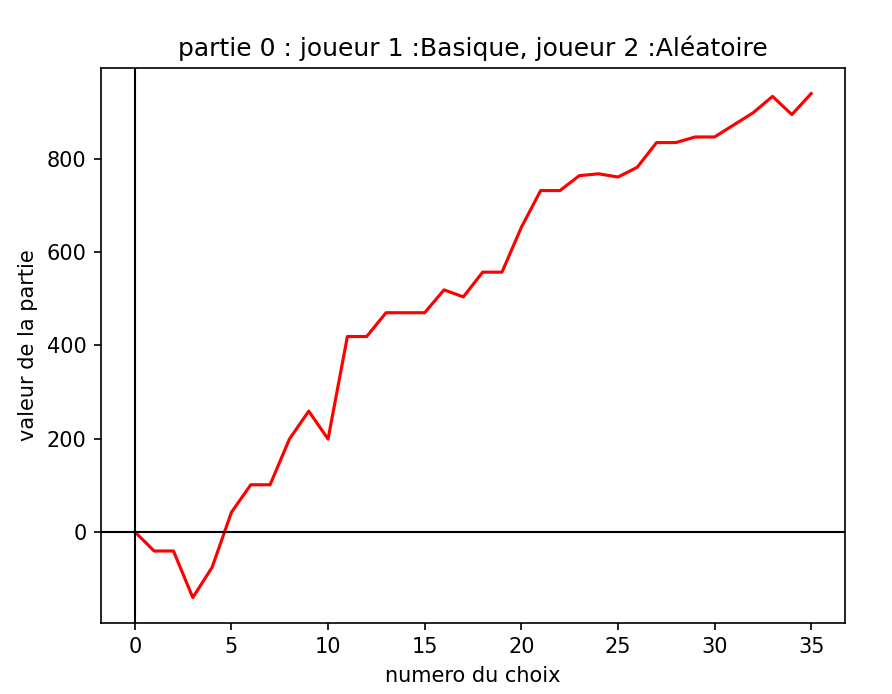
\includegraphics[width=4cm,height=4cm]{graphiques/valeur_basique_alea1}

				Seconde partie:

				Evolution de la valeur (l'agent qui utilise les règles est l'agent nommé basique en joueur 1 donc en max):

				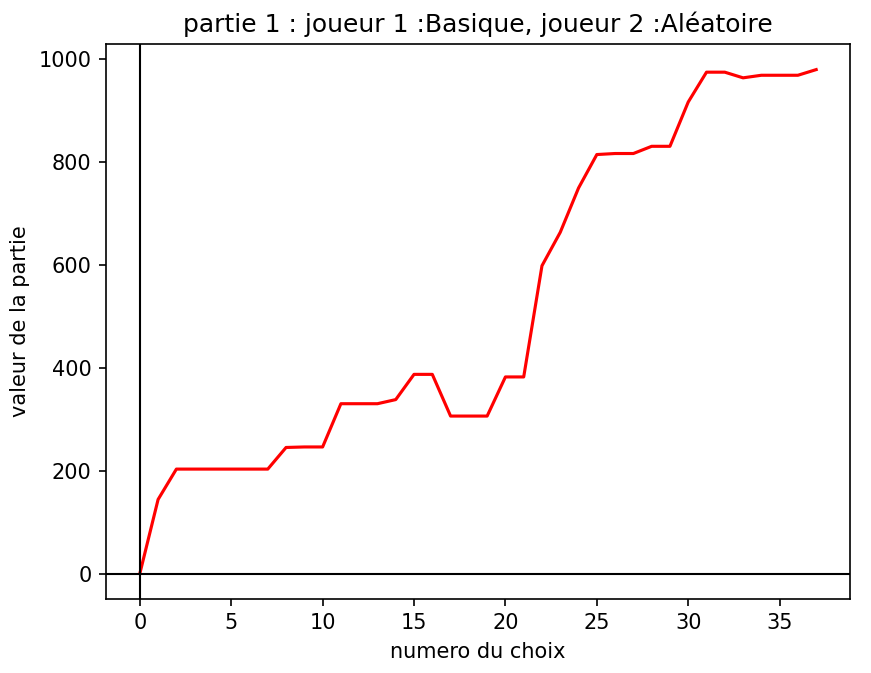
\includegraphics[width=4cm,height=4cm]{graphiques/valeur_basique_alea2}

				Le temps de réponse ne semble pas dépendre de la phase de la partie. Voici le temps de réponse au cours des 30 parties mises bout à bout:

				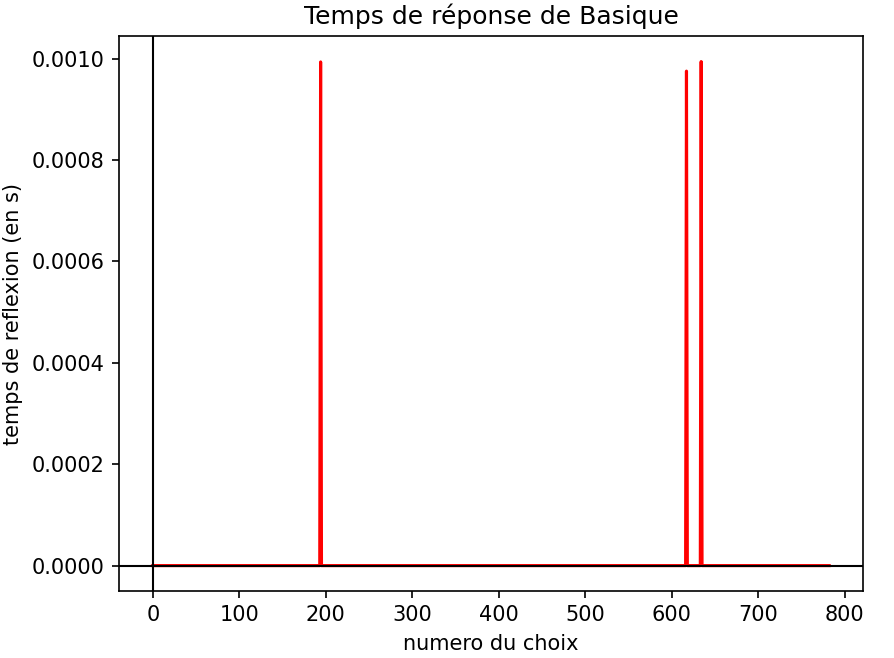
\includegraphics[width=4cm,height=4cm]{graphiques/temps_basique_alea1}

			\paragraph{Avantages :}
				Le temps de réponse et trés court. L'ia est trés forte contre des agents de bas niveau car elle cherche le plus possible à faire des dêgats.
			\paragraph{Défaults :}
				Le jeu pokemon et trop compliqué pour qu'un jeu de règles soit suffisant pour y être performant. Ces règles ne permettent pas de prendre en compte les 					spécificités de l'etat du jeu à un moment donné de la partie. Une règle qui est valable dans certaines situation peut être une grande erreur dans d'autres. Par 							exemple, changer de pokemon à chaque fois qu'il y a un désavantage de type n'est pas une bonne idée. Si le pokemon de l'adversaire a trés peu de PV et qu'on 					est plus rapide que lui, il vaut mieux attaquer pour le mettre KO car ainsi il ne pourra pas riposter (étant plus lent, l'adversaire attaque en second et ne pourra 						pas attaquer si il est mit KO). L'agent resultant a donc un comportement trés prévisible qui peut être anticipé par un adversaire humain et il a une trés 								mauvaise adaptation aux situations. 

				L'agent cherche en priorité à mettre des dêgats mais ne profite pas des avantages que représentent les bonus et les statuts. 

				Il faut avoir une bonne connaissance du jeu pour trouver des règles convenables. Donner des règles sur l'utilisation des statuts et des bonus est par exemple 							difficile commes ces éléments sont trés situationnels. Le choix du premier pokemon est aussi difficile.

				L'ia obtenue n'est pas généralisable et ne peut pas être réemployée dans des jeux similaires.
		\subsubsection{Minimax}
			L'algorithme du minimax est un algorithme pour les jeux à deux joueurs en tour par tour à choix alternés. Dans cet algorithme on considère que un joueur le max 						cherche à maximiser la valeur du jeu et un autre cherche à la minimiser.
			Dans cet algorithme, l'ordinateur visite l'arbre du jeu sur une certaine profondeur puis remonte les valeurs associées à chaques coup de la manière suivante :
			\begin{itemize}
				\item Si on est à la profondeur p ou si le jeu est fini, on renvoie une aproximation de la valeur du jeu (celle de la fonction d'évaluation).
				\item Si c'est au min de jouer, il choisit l'action qui minimise la valeur du jeu.
				\item Si c'est au max de jouer, il choisit l'action qui maximise la valeur du jeu.
			\end{itemize}

			Une amélioration de cet algorithme est l'algorithme alpha beta qui stocke en mémoire deux entiers, alpha et beta, qui stockent respectivement la plus grande valeur 						trouvée par le max et la plus petite trouvée par le min et permet d'élaguer l'arbre c'est à dire de ne pas visiter les branches qu'il est inutile de visiter (celle qui quoi 						qu'il arrive ne seront pas choisies par l'adversaire.)

			Notre objectif dans cette section va être de discuter d'une adaptation de l'algorithme alpha beta au jeu pokemon.
			
			\paragraph{Problème de l'ordre de jeu et de l'atomicité des tours:}
				L'ordre de jeu dans pokemon n'est pas alternatif car un choix peut être demandé aux deux joueurs ou à un seul (en cas de KO) sans ordre prédéfinit. Il faut 							donc passer par une fonction intermédiaire qui regarde qui doit jouer et :
				\begin{itemize}
					\item Si un seul joueur doit jouer, on applique l'algorithme du minimax habituel.
					\item Si deux joueurs doivent jouer, le choix de l'agent sera pour celui qui est \emph{le plus optimal quel que soit le choix de l'adversaire}.
				\end{itemize}
			    \smallskip    			Pour determiner quel est le choix \emph{le plus optimal quel que soit le choix de l'adversaire}, on parcourt les mouvements de disponibles pour l'agent et on applique 				l'algorithme du minimax habituel en considérant cette action comme choisie. Pour chaque mouvement l'adversaire va donc choisir l'action qui est la meilleure sachant 					que notre agent à choisit ce mouvement, il va choisir le meilleur contre à notre action. On va récupérer une valeur d'état associée à chaque mouvement et son 						meilleur contre (comme les 2 joueurs jouent, il faut deux actions pour déplacer l'etat) et en déduire la meilleure action.
    
    			Par exemple pour le max : On parcourt l'ensemble des actions disponibles pour le max. Pour chaque action, le min choisit l'action qui minimise la valeur de l'etat 						sachant l'action qui est jouée par le max. On recupére toutes les valeurs associées aux couples mouvements du max, meilleur contre du min et on choisit le couple qui                                                          
    			a la valeur la plus grande. Ainsi on a choisit l'action qui maximise la valeur de l'état même si le min choisit le meilleur contre de cette action.
    			
    			L'algorithme sera developpé de la même manière que le minimax habituel mais avec trois fonction qui s'entre-appellent au lieu de deux : il y aura la \emph{fonction interface}, la fonction \emph{min} et la fonction \emph{max}.
			\paragraph{Problème de la Stochasticité}
			    Comme nous l'avons vu dans la section 5.1.2, le jeu pokemon n'est pas un jeu déterministe. Cependant, dans un premier temps, nous considèreront que le facteur chance est négligeable. Cette agent traitera donc l'aléatoire de la manière suivante : lorsqu'un etat peut mener à plusieurs états différents via un facteur chance, un de ces états sera choisit en respectant les probabilités qui sont associées à chaque état. L'etat choisit sera considéré comme le seul etat possible, ce qui menera forcement à des erreurs dans l'évaluation de la valeur des futurs états.
            \paragraph{Implementation:}
                
                La classe \emph{JoueurMinimax} (tout les agents qui utilisent le minimax en héritent)(source : joueurs.py):
                
                \lstinputlisting[language=Python, tabsize=1,basicstyle=\scriptsize , linerange=JoueurMiniMax-end,includerangemarker=false]{code/joueurs.py}
                
                L'agent (source : joueurs.py):
                
                \lstinputlisting[language=Python, tabsize=1,basicstyle=\scriptsize , linerange=JoueurAlphaBeta1-end,includerangemarker=false]{code/joueurs.py}
                
                L'algorithme minimax (source : minimax.py): 
                \smallskip
				La fonction interface (on ne met que celle du joueur 1, celle du joueur 2 étant similaire mais inversée):
					    \lstinputlisting[language=Python, tabsize=1,basicstyle=\scriptsize , linerange=interface-end,includerangemarker=false]{code/minimax.py}
					    
				La fonction max (source : minimax.py): 
					    \lstinputlisting[language=Python, tabsize=1,basicstyle=\scriptsize , linerange=max-end,includerangemarker=false]{code/minimax.py}
				\smallskip
				La fonction de traitement de l'aleatoire (source : minimax.py): 
				\lstinputlisting[language=Python, tabsize=1,basicstyle=\scriptsize , linerange=alea-end,includerangemarker=false]{code/minimax.py}
			\paragraph{Résultats :}
			    Le coût des calculs et le facteur de branchement limite la recherche à 2 de profondeur ce qui reste interréssant étant donné que dans la plupart des coups, il faut regarder les mouvements possibles pour les deux joueurs (à cause de l'atomicité des tours).
			    
			    L'agent obtenu est plus performent que tout les agents précédents.
			    
			    Son temps de réponse est bien plus élevé que ceux des agent précedents(entre 3 en 20s).
			    Contrairement aux agents précédents, son temps de réponse depend de la phase de la partie. En fin de partie il y a moins de choix possibles donc moins de calculs à faire.
			    
			    Son comportement est trés cohérent ce qui est une bonne réussite car on ne lui a pas donné d'instruction préalable. Dans la plupart des cas il change de pokemon quand il y a un désavantage de type mais pas quand son adversaire est affaiblit et qu'il peut le finir parce qu'il est plus rapide. Quand il a un avantage il attaque. Il lui arrive d'utiliser des statuts comme la paralysie et vampigraine, et des bonus.
			    
			    Même si il bat l'IA basique, certaines partie contre cet agent sont trés sérrées car il lui arrive de faire des érreurs à cause du facteur chance.
			    
			    Le pokemon qu'il choisit en premier est pikachou. C'est un trés bon choix car il est rapide et il possède l'attaque change éclair qui lui permet de changer de pokemon tout en faisant des dêgats au cas où il serait en désavantage de type.
			    
			    Face à un humain, l'agent commence à être interressant : il bat les débutants et peut mettre en difficultée les joueurs intermédières (Exemple la première partie faite par un des concepteur contre cette ia n'a été gagné avec un seul pokemon restant).
			    
			    Voici un exemple de partie contre l'aléatoire:
			    
			    La valeur de la partie (l'agent est en position de max):
			    
			    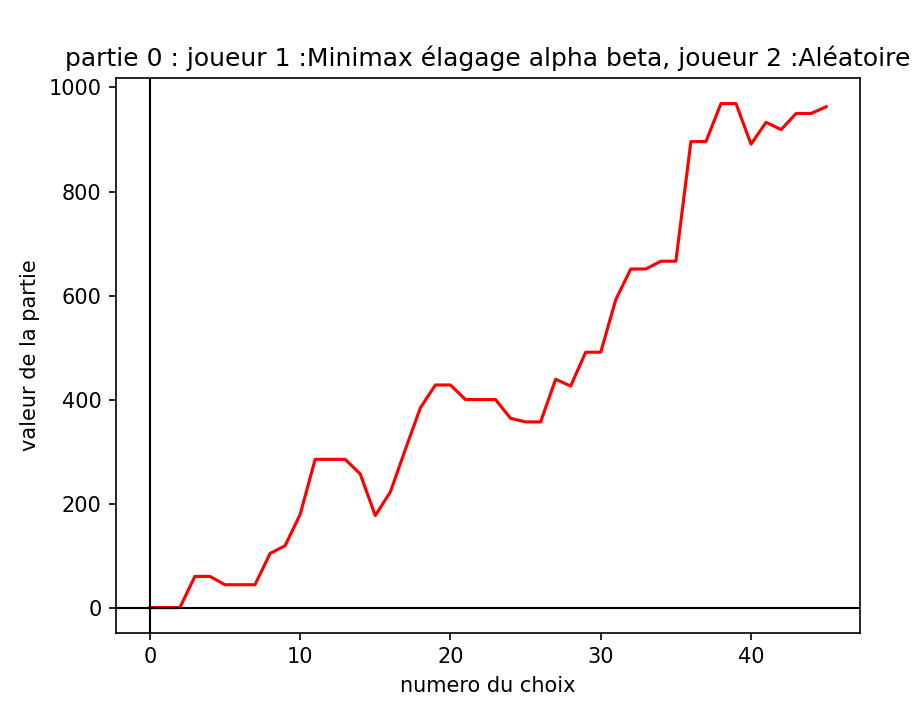
\includegraphics[width=4cm,height=4cm]{graphiques/valeur_alphbet_alea1}
			    
			    Le temps de réponse: On voit bien sur le graphique qu'il diminue en fin de partie.
                
                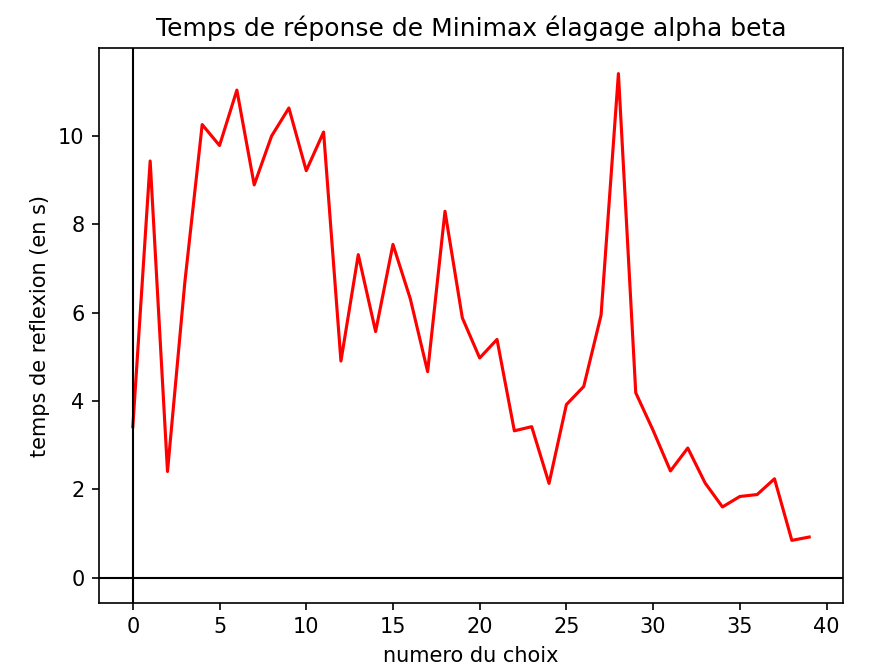
\includegraphics[width=4cm,height=4cm]{graphiques/temps_alphbet_alea1}
                
                Voici des exemples de partie contre l'ia basique (agent avec un jeu de règle):
			    
			    Deux exemples de la valeur de la partie (l'agent est en position de max):
			    
			    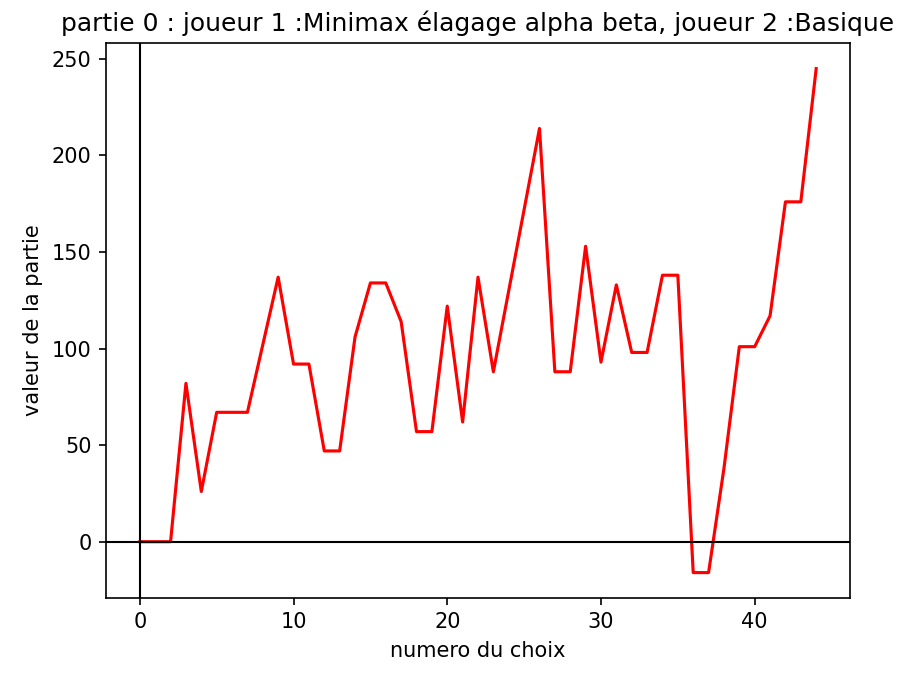
\includegraphics[width=4cm,height=4cm]{graphiques/valeur_alphbet_basique1}
			    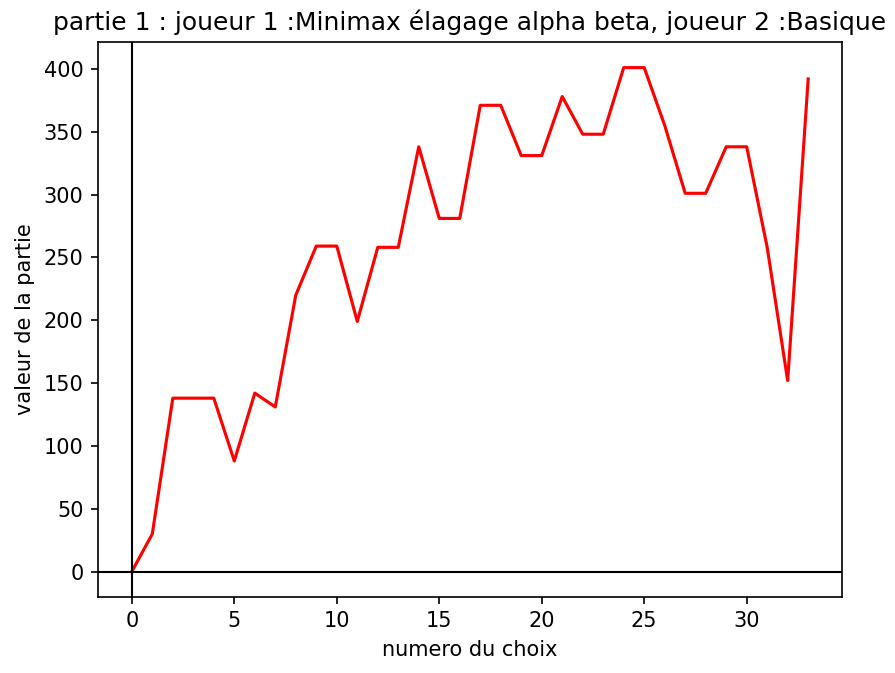
\includegraphics[width=4cm,height=4cm]{graphiques/valeur_alphbet_basique2}
			    
			    Un exemple de temps de réponse contre l'ia basique:
                
                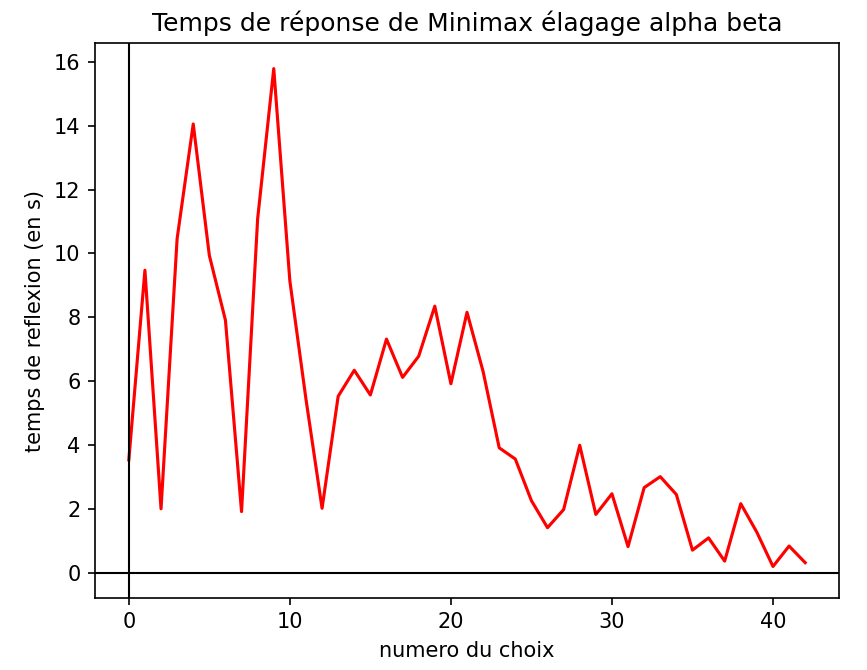
\includegraphics[width=4cm,height=4cm]{graphiques/temps_alphbet_basique1}
            \paragraph{Avantages :}
                L'agent n'est pas prévible comme il ne suit pas un jeu de règles.
                
                Il ne necessite pas de connaissance particulières dans le jeu et est généralisable à tout les jeux similaires à pokemon (jeu avec atomicité des tours et Stochasticité).
                
                Il est plus performant que tout les agents précédents et surtout en fin de partie.
                
                L'agent n'utilise pas que des attaques qui font des dêgats à court terme, il utilise aussi des statuts et des bonus.
            \paragraph{Desavantages :}
                Le temps de réponse de l'agent est assez important. Si on voulait créer une application dans laquelle des joueurs jouent contre notre ia, il serait difficile de leur faire accepter ce delai.
                
                L'agent à du mal à traiter l'aléatoire ce qui l'amène à faire des erreurs.
                
                La faible profondeur de recherche limite la comprehension réelle de l'état du jeu et empêche l'utilisation d'attaques à trés long terme comme piège de rock
                
                L'agent est trés prévisible en début de partie, sachant qu'il prend toujours pikachou en premier, l'adversaire peut choisir son contre.
                
        \subsubsection{Expectiminimax}
            Dans cette section on va apporter une amélioration à l'algorithme alpha beta afin de mieux traiter le facteur chance : l'expextiminimax.
            Pour ce faire, nous allons simplement changer la fonction de traitement de la chance : à chaque foix qu'il y aura plusieurs états possibles pour une action, la valeur de cette action sera l'esperance des valeurs de tout les états.
            \paragraph{Implementation:}
                
                Seule la fonction de traitement de l'aléatoire change:
                
                L'agent (source : joueurs.py):
                
                \lstinputlisting[language=Python, tabsize=1,basicstyle=\scriptsize , linerange=JoueurAlphaBeta2-end,includerangemarker=false]{code/joueurs.py}
                
                La fonction de traitement de l'aleatoire (minimax.py):
                
                \lstinputlisting[language=Python, tabsize=1,basicstyle=\scriptsize , linerange=esperance-end,includerangemarker=false]{code/joueurs.py}
                
            \paragraph{Résultats :}
                Le temps de reponse est plus élevé car il faut traiter en plus les branches liées à la chance. Il faut en général entre 10 et 30 secondes pour repondre. Cependant contrairement à l'agent précédent, il arrive que le temps de réponse l'ia expectiminimax stagne voire augmente en fin de partie. L'explication c'est qu'en fin de partie il y a plus de branches liées à la chance. L'augmentation du nombre de branches liées à la chance s'explique par l'augmentation du nombre de situation ou les deux pokemon sur le terrain ont des statuts. En effet, dans ce cas là, si les deux pokemons ont la même vitesse, la chance est à utilisée une première fois pour determiner qui attaque en premier et une seconde fois pour determiner qui subit les statuts en premier. Il y a donc plus de quatres etats possibles.
                
                Ensuites, les performances de l'agent sont superieures. En effet, grâce à sa maitrise du facteur chance cet agent bat tout les agents précédents.
                
                Les agents alea et basique sont battuts avec un écart de PV trés élevé mais en plus de tour qu'il n'en failait à l'agent minimax pour les battre. Cela montre que l'agent expectiminimax prend moins de risque mais au final est plus précis.
                
                Comme pour l'agent précédent, l'agent expectiminimax choisit pikachou en premier ce qui semble confirmer que c'est un bon choix.
                
                Son comportement et plus cohérent que tout les agents précédents car il ne fait pas d'erreurs liées au facteur chance.
                
                Face à un humain, l'agent est interressant : il bat les débutant et peut mettre en difficultée voire battre les joueurs intermédières.
                
                Voici un exemple de partie contre l'ia basique (agent avec un jeu de règle):
			    
			    La valeur de la partie (l'agent est en position de max) est à droite et le temps de réponse à gauche (On est dans le cas ou il ne diminue pas en fin de partie):
			    
			    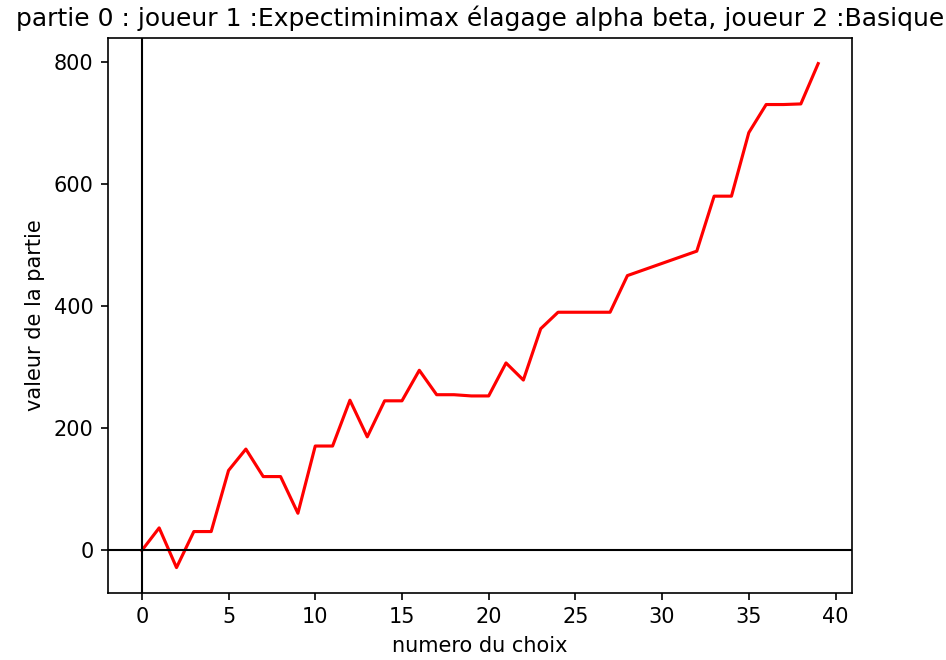
\includegraphics[width=4cm,height=4cm]{graphiques/valeur_alphbet2_basique1}                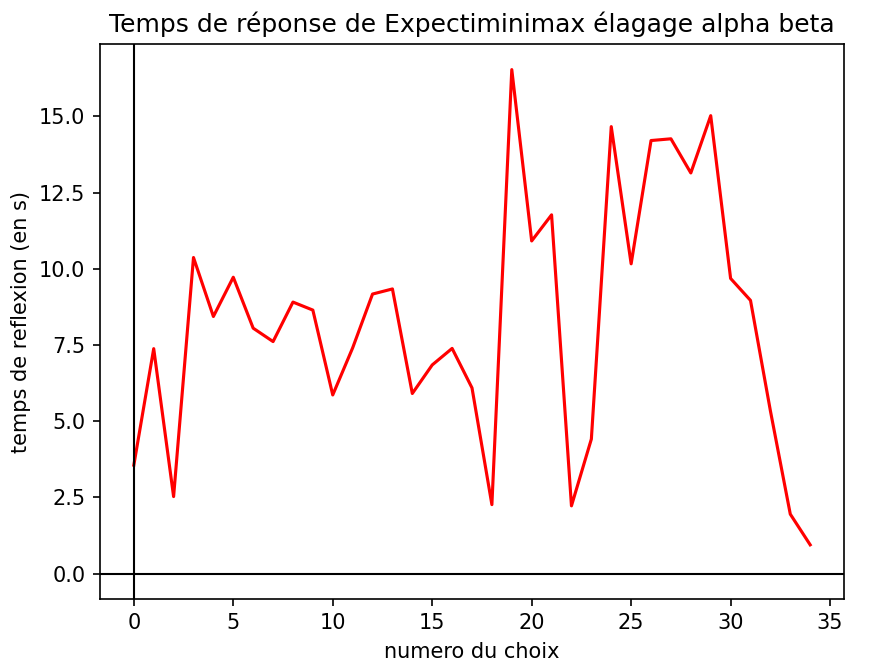
\includegraphics[width=4cm,height=4cm]{graphiques/temps_alphbet2_basique1}
                
                Voici deux exemples de partie contre l'ia alpha beta classique:
			    
			    Les valeur de la partie (l'agent expectiminimax est en position de max):
			    
			    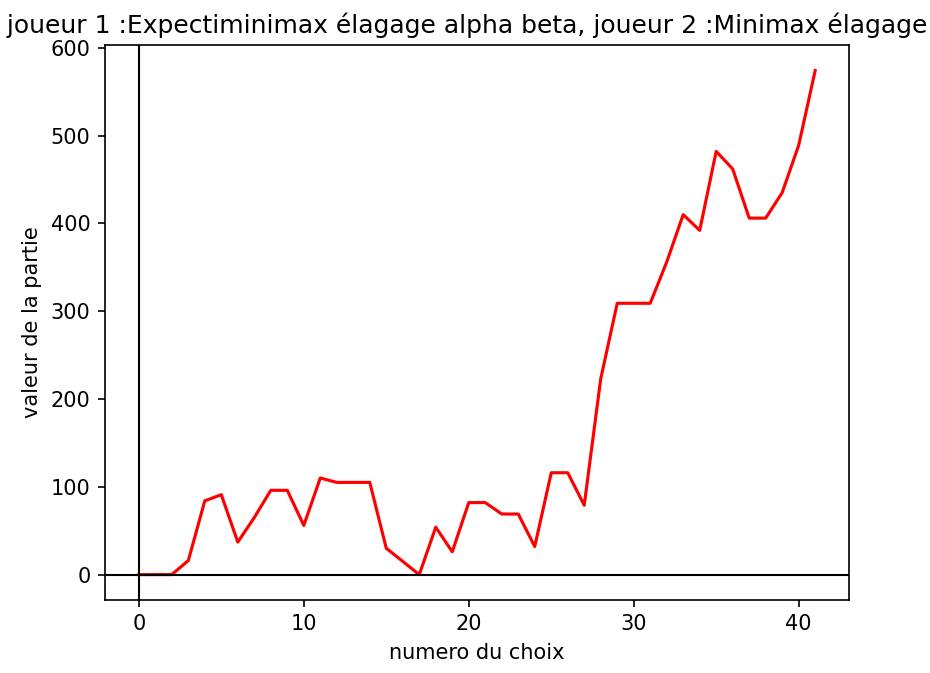
\includegraphics[width=4cm,height=4cm]{graphiques/valeur_alphbet2_alphabet1}
			    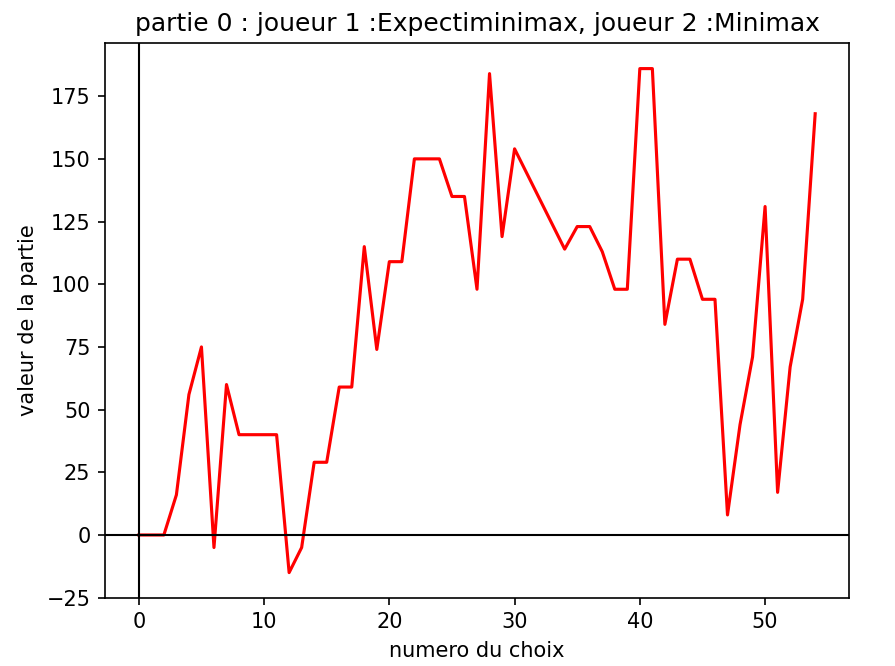
\includegraphics[width=4cm,height=4cm]{graphiques/valeur_alphbet2_alphabet2}
			    
			    Un exemple de temps de réponse: Cette fois il diminue bien en fin de partie.
                
                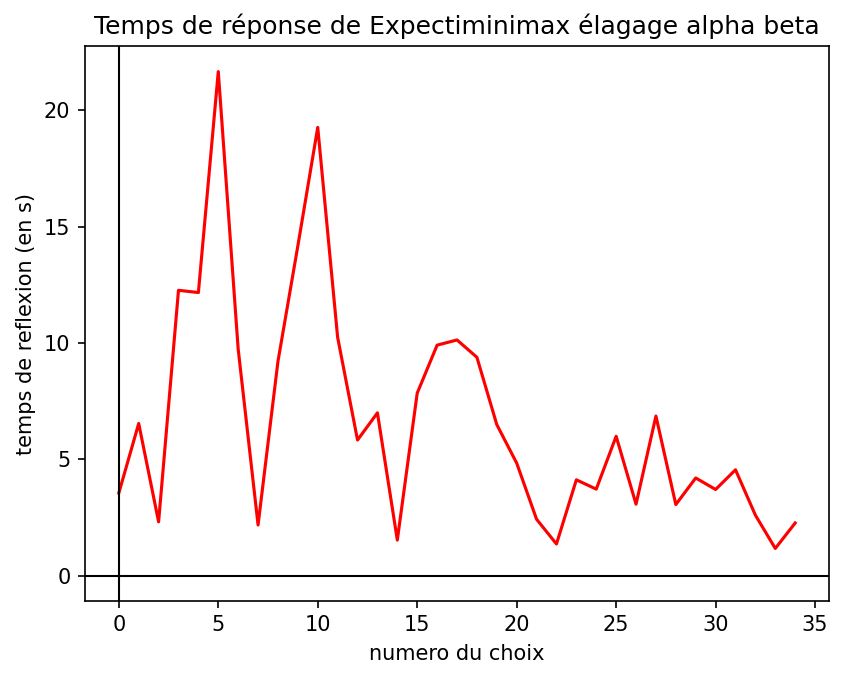
\includegraphics[width=4cm,height=4cm]{graphiques/temps_alphbet2_alphabet1}
            \paragraph{Avantages :}
                L'agent prend mieux en compte le facteur chance et fait moins d'erreurs.
                
                La solution proposée est toujours aussi générale, elle peut s'appliquer à tout les jeux à information parfaite, avec atomicité des tours.
            
            \paragraph{Desavantages :}
                Cette amélioration s'est faite au prix d'une augmetation du temps de réponse. 
                
                La faible profondeur de recherche reste une limite importante.
                
                L'agent est trés prévisible en début de partie, sachant qu'il prend toujours pikachou en premier, l'adversaire peut choisir son contre.
                
        \subsection{Ordre des mouvements}
            L'ordre de traitement des mouvements a une importance capitale pour l'élagage alpha beta. Plus un noeud correspondant à une valeur élevée est visité tôt, plus il entrainera de coupures.
            Une pratique habituelle pour trier les mouvements est de faire une recherche superficielle (c'est à dire utiliser l'algorithme du minimax avec une profondeur de 1), avant d'appliquer l'algorithme du minimax.
            \paragraph{Implementation :}
                \lstinputlisting[language=Python, tabsize=1,basicstyle=\scriptsize , linerange=tri\_mvt-end,includerangemarker=false]{code/jeu.py}
            \paragraph{Resultat :}
                Dans le cas de notre jeu, une recherche superficielle demande trop de calculs par rapport au temps gagné par les coupures suplémentaires qu'elle entraine.
                Ainsi, on observe pour tout les agents utilisant le minimax, une augmentation du temps de recherche lorsqu'on trie au préalable à la profondeur 0. 
                (Pour trier à la profondeur 0, il faut donner à la variable condition\_tri l'expression : lambda profondeur : profondeur <=1 au lieu de lambda p : False).
                Exemple : Voici le temps de reponse de l'agent expectiminimax contre l'agent minimax, avec tri à droite et sans tri à gauche.
            
            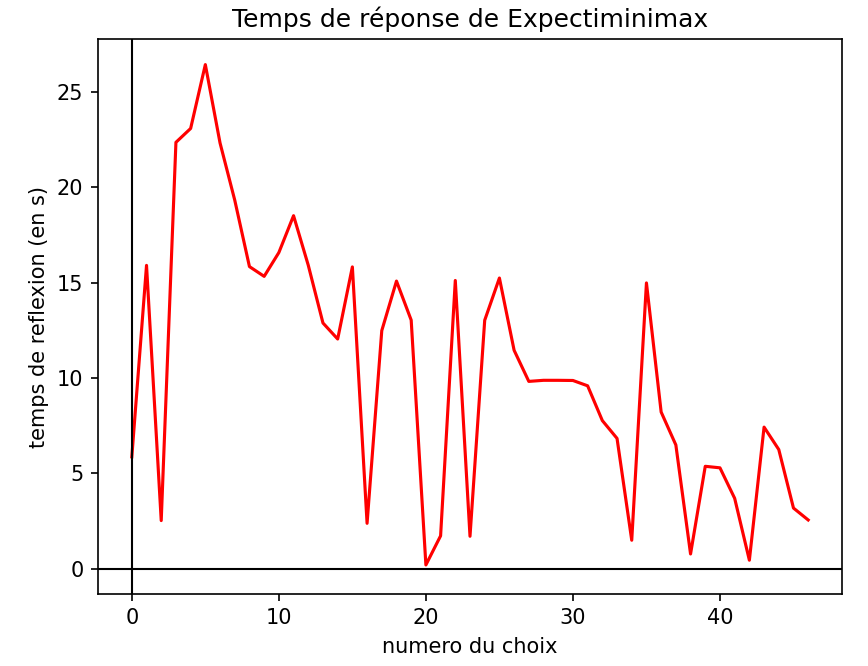
\includegraphics[width=4cm,height=4cm]{graphiques/temps_alphbet2_alphabet_tri}
            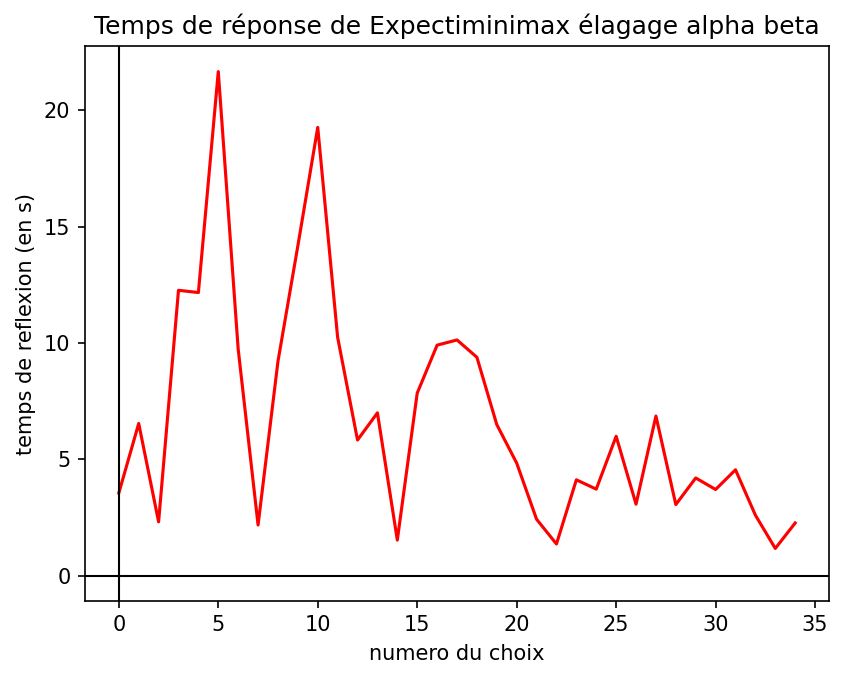
\includegraphics[width=4cm,height=4cm]{graphiques/temps_alphbet2_alphabet1}
            
            On voit que avec le tri les délais sont plus long. On trouve des résultats similaire pour l'agent minimax.
    \subsection{Solutions Envisageables}
        Deux mois de projet c'est une longue periode pour un projet scolaire, mais avec un sujet aussi vaste, il reste toujours des pistes à creuser, des détails à peaufiner. Cette section sera donc dédiée à des pistes que nous aurions voulu explorer sans pour autant avoir le temps de le faire.
        \subsubsection{Ordre des mouvements}
            Un des plus grand défaults des ia les plus performentes que nous avons réussit à coder est le temps de reponse. 
            Avec un temps de réponse plus court, on pourrait soit améliorer l'experience utilisateur, soit augmeter la profondeur de recherche et avoir une ia plus performante.
            Ainsi, pour les améliorer nos ia, un bon tri des mouvements avant les recherches serait interressant. Pour cela, on pourrait utiliser deux choses :
            \begin{itemize}
				\item Un table de hashage qui stocke les mouvements les plus efficaces qui sont a tester en premier.
				\item Lorsque deux etats ne différent que de par un facteur chance et qu'on a déjà fait l'algorithme du minimax pour le premier, on peut stocker le mouvement résultant et l'explorer en premier. Souvent deux etats qui ne différent que d'un facteur chance sont trés proches et le mouvement stocké sera le bon créant donc de nombreuses coupures.
			\end{itemize}
		\subsubsection{Recherche de principale variation}
		    Toujours dans l'idée de réduire le temps de calcul, on pourrait se pencher sur un amélioration de l'algorithme alpha beta qui est nommé recherche de principale variation ou PVS (Principal Variation Search).
		    C'est un algorithme qui repose sur un bon tri préalable des mouvements c'est pourquoi le point précédent sera important.
		    Il se déroule de la manière suivante:
		    \begin{itemize}
				\item On tri les mouvements disponibles.
				\item Pour le premier mouvement on fait une recherche complète avec l'algorithme minimax
				\item Pour tout les autres on fait une recherche de fenetre nulle (zero window search). C'est une recherche pour laquelle beta = alpha + 1. Ce type de recherche produit bien plus de coupure que l'élagage alpha beta et ne renvoie qu'une information : est-ce que le mouvement améliore la valeur actuelle.
				\item Pour tout les mouvements qui ont améliorer la valeur actuelle, on effectue une recherche complète.
				\item On remonte la valeur de la recherche complète qui est la plus grande pour le max et la plus petite pour le min.
			\end{itemize}
			Ainsi, si l'ordre des mouvements est bon on aura fait trés peu de recherches complètes et une majorite de recherches à fenetre nulle et on aura économiser un temps précieux.
        \bigskip
        \section{interfaces}
    \subsection{Introduction}
        Pour représenter notre jeu, nous avons donc créer 2 interfaces: une interface textuelle et une interface graphique. Afin de faciliter la transition entre ces deux interfaces et le programme du jeu, qui est donc le même peut importe l'interface, nous avons décidé de faire en sorte qu'elles aient toutes les deux la même structure. Elles sont ainsi simplement différentes dans la façon dont elles récupèrent/affichent les informations. C'est au début de la partie que l'une ou l'autre seront choisie par l'utilisateur via la console.
    \subsection{Interface Textuelle}
        Lorsque c'est l'interface textuelle qui est choisie, l'entièreté de la partie se déroulera alors dans la console, que ce soit les choix des joueurs ou les informations sur le déroulé du jeu. Au cours de la partie, les différents choix à effectuer par le/les joueurs humain(s) si il y'en a seront à taper directement dans la console (pour les ia seuls les résultats de leurs choix s'afficheront).
        Dans le cas de l'interface textuelle, une fonction 'input securise' assure la bonne comprehension des reponses des utilisateurs. Celle-ci ne laissent passer que des réponses pré-definies (ex: un nom de pokemon, un nom d'attaque) et permet ainsi d'éliminer les erreurs dûes aux réponses non-conformes des utilisateur (nom mal orthographié ou inexistant).
        \bigskip
            \subsubsection{déroulé d'un tour}
                Dans un premier temps, il faudra taper dans la console la nature des deux joueurs ainsi que leurs nom et leur pokemon de départ, en répondant aux questions correspondantes dans la console comme explicité ci-contre:(cf image 1 au point 6.2.2)
                
                \bigskip
        
                Pour chaque tour (après un récapitulatif des choix respectifs des deux joueurs si il s'agit du premier tour), les deux joueurs sont appelé à choisir ce qu'ils vont faire, en choisissant entre attaquer ou changer de pokemon, avec la possibilité d'avoir accès aux informations de la partie avant de choisir. Les différents choix d'attaque ou de pokemon posssible seront rappelés au joueur avant qu'il ne choisisse. Voici des exemples :(cf image 2 au point 6.2.2)
    
                \bigskip
    
                A la fin du tour, un résumé des différents actions ayant eu lieu durant ce tour sera affiché dans la console, accompagné d'un bilan global de l'état du jeu à ce tour, avec les informations sur les pokemons des deux joueurs commme présenté ci-contre:(cf image 3  au point 6.2.2)

                \bigskip

                Enfin, lorsque qu'un joueur n'a plus de pokemon en état de combattre, un message vient annoncer le vainqueur et la fin de la partie.(cf image 4  au point 6.2.2)

            \bigskip
            
            \subsubsection{affichages en textuel:}
                Touts les affichages de l'interface textuelle sont gérés par des print appliqués par les différentes fonction de la classe InterfaceTexte ou par le fichier jeu (voir architecture du programme) pour ce qui concerne les informations destinées aux utilisateur et par la fonction 'input securise' pour ce qui concerne les informations données par l'utilisateur au programme.
                
                
                Voici quelques capture d'écran d'une partie avec l'interface textuelle.
                
                Image 1: début de partie
                
                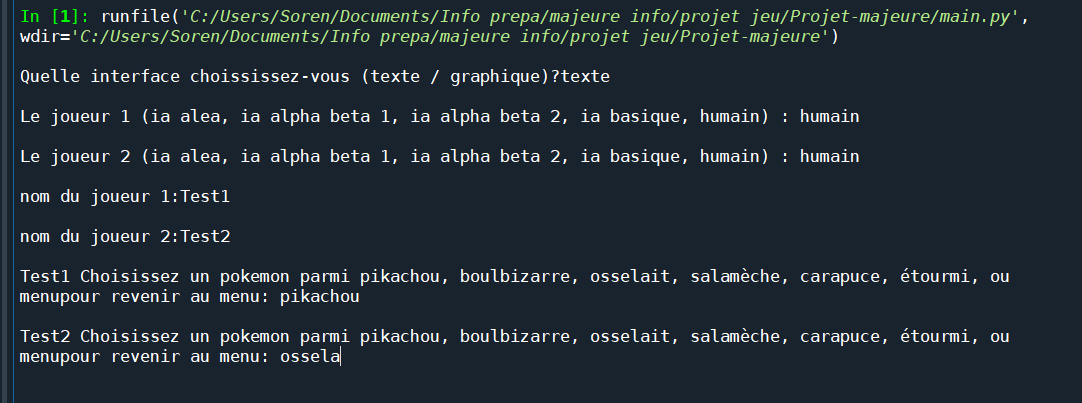
\includegraphics[width=16cm,height=6cm]{images/text1}

                Image 2: Choix lors d'un tour
                
                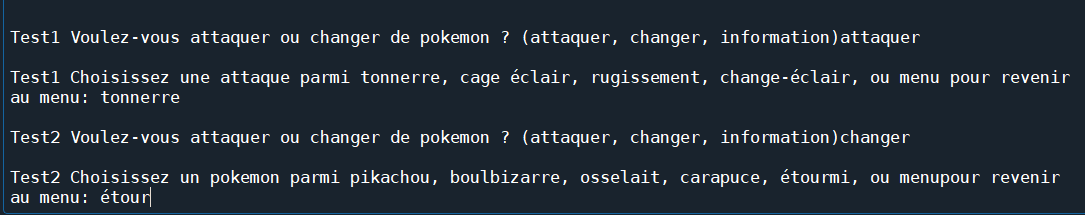
\includegraphics[width=16cm,height=6cm]{images/text2}

                Image 3 : Fin du tour
                
                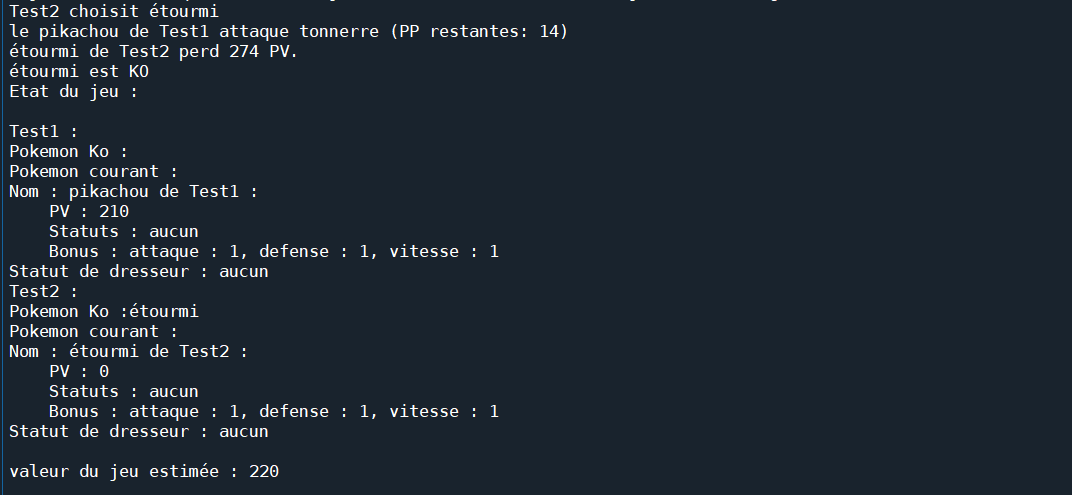
\includegraphics[width=16cm,height=6cm]{images/text3}

                Image4 : Fin de la partie
                
                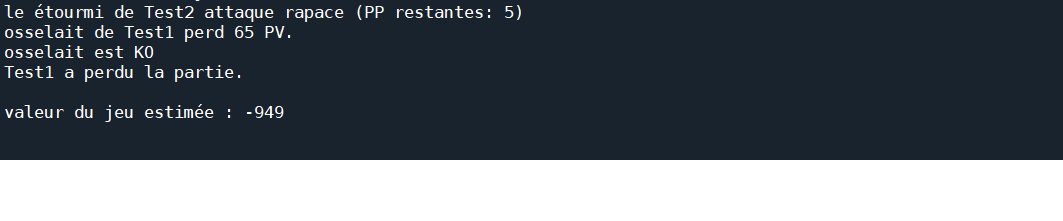
\includegraphics[width=16cm,height=6cm]{images/text4}
                

            \bigskip
    \subsection{Interface Graphique}
        L'interface graphique reprends donc la même structure que l'interface textuelle. Cependant, dans le cas de l'interface graphique, le joueur éffectue ses choix via des boutons ou des zones de texte apparaissant sur la fenêtre du jeu et non plus directement via la console. Le jeu se joue donc sur une fenêtre générée par le programme avec, sur la partie gauche, un decor ou apparaissent les pokemons actuels des deux joueurs ainsi qu'une partie sur la droite servant pour effectuer les choix/afficher les informations relatives au jeu. La nature de ces parties vous sera détaillée dans le point 6.3.2.
        Afin de pouvoir récupérer les choix des joueurs, on utilise les fonctions waitvariable et waitwindow qui nous permettent, via les fonctions liées aux boutons qui affectent ainsi une certaine valeure a la variable récupérée par le programme, de mettre celui-ci en suspent tant que le bouton n'est pas cliqué. 
        
        
        
        \subsubsection{déroulé d'un tour}
            Comme pour l'interface textuelle, il faut d'abord définir le type, le nom et le premier pokemon des deux joueurs. Pour le type et le premier pokemon, un simple clic sur le bouton voulu suffit. Pour ce qui est du nom, une zone de texte apparaît avec 'nom du joueur' en valeure par défaut. Il suffit de supprimer ce texte, de taper le pseudo voulut et d'appuyer sur la touche 'entrée' du clavier pour valider.(cf image 1, 2, 3 au point 6.3.2)

            \bigskip

            Pour chaque tour (un récapitulatif des choix respectifs des deux joueurs apparait quelques secondes si il s'agit du premier tour), comme pour l'interface textuelle, les deux joueurs choisissent entre attaquer, changer, ou avoir des informations avant de faire ce choix. Ici, ces choix se gèrent grâce à des boutons à cliquer.(cf image 4, 5, 6, 7 au point 6.3.2)

            \bigskip

             Une fois ces choix éffectués, ils s'appliquent et un récapitulatif des actions réalisées et des nouvelles informations apparaît pendant quelques secondes.(cf image 8 au point 6.3.2)

             \bigskip

             Enfin, lorsque qu'un joueur n'a plus de pokemon en état de combattre, les informations récapitulant le dernier tour apparaissent avec un message annoncant le vainqueur et la fin de la partie.(cf image 9 au point 6.3.2)

             \bigskip
            
        \subsubsection{affichages graphiques:}
            La fenêtre générée est crée via le module Tkinter. Elle est composée de 2 frames, une grande à gauche et une autre plus petite à droite. Dans notre programme, la fenêtre est définie dans le fichier fenêtre avant d'être initialisée en tant qu'attribut de la classe InterfaceGraphique. Nous tenons à préciser que nous avons essayé de reprendre au mieux l'interface de combat graphique des jeux pokemons originaux ainsi que des images issus des premiers jeux de la license pour ce qui concerne les pokemons et le decor notamment.
            \begin{itemize}
                \item La grande frame de gauche est dédiée au décor du jeu. Elle contient un grand canva qui la recouvre entièrement, dans lequel on implémente l'image servant de paysage de fond à notre jeu. Sur ce canva sont disposés, lors du choix des pokémons, 2 canvas contenant les images (sprites) des pokemons des deux joueurs. Le joueur 1 se situe en bas à droite, de dos, tandis que le joueur 2 se situe en haut à gauche, de face.Lors d'un changement de pokemon, le canva du pokemon concerné est détruit et remplacé par un nouveau contenant le nouveau pokemon.

                \item La frame de droite, elle, sert d'interface entre l'utilisateur et le jeu et d'endroit pour afficher les informations du jeu. Cette frame est en réalité un objet d'une des classes ci-dessous:
                \begin{itemize}
                    \item IHM, frame permettant de faire le choix attaquer, changer ou information.
                    \item Attaquef, frame correspondant au choix attaquer.
                    \item Changerpoke, frame correspondant au choix de changer de pokemon.
                    Information, frame correspondant au choix information.
                    \item Demandernom, frame correspondant au choix de pseudo en début de partie.
                    \item Choixjoueur, frame correspondant au choix du type de joueur en début de partie.
                    \item Etatjeu, frame affichant l'etat du jeu entre les tours.
                \end{itemize}
                A chaque changement de frame, celle-ci est détruite puis remplacée par une nouvelle instance d'une des classes ci-dessus.
            \end{itemize}
            
            \bigskip

            Pour ce qui est des boutons, ils sont crées via Tkinter et sont liés à une fonction qui permet d'affecter une certaine valeure à l'attribut 'choix' de la fenêtre qui est par la suite récupérée et traitée par l'interface. Le fonctionnement est simililaire pour le champs de texte permettant de renseigner le pseudo des joueurs en début de partie, qui est un Widget Entry de Tkinter affectant la valeure reçue lors de la pression de la touche 'entrée' à l'attribut 'choix' de la fenêtre.

            Voici quelques images pour l'interface graphique:
            Image 1: début de partie
        
            \includegraphics[width=13cm,height=7cm]{images/debut\_partie}
            
            Image 2 : choix des noms :
            
            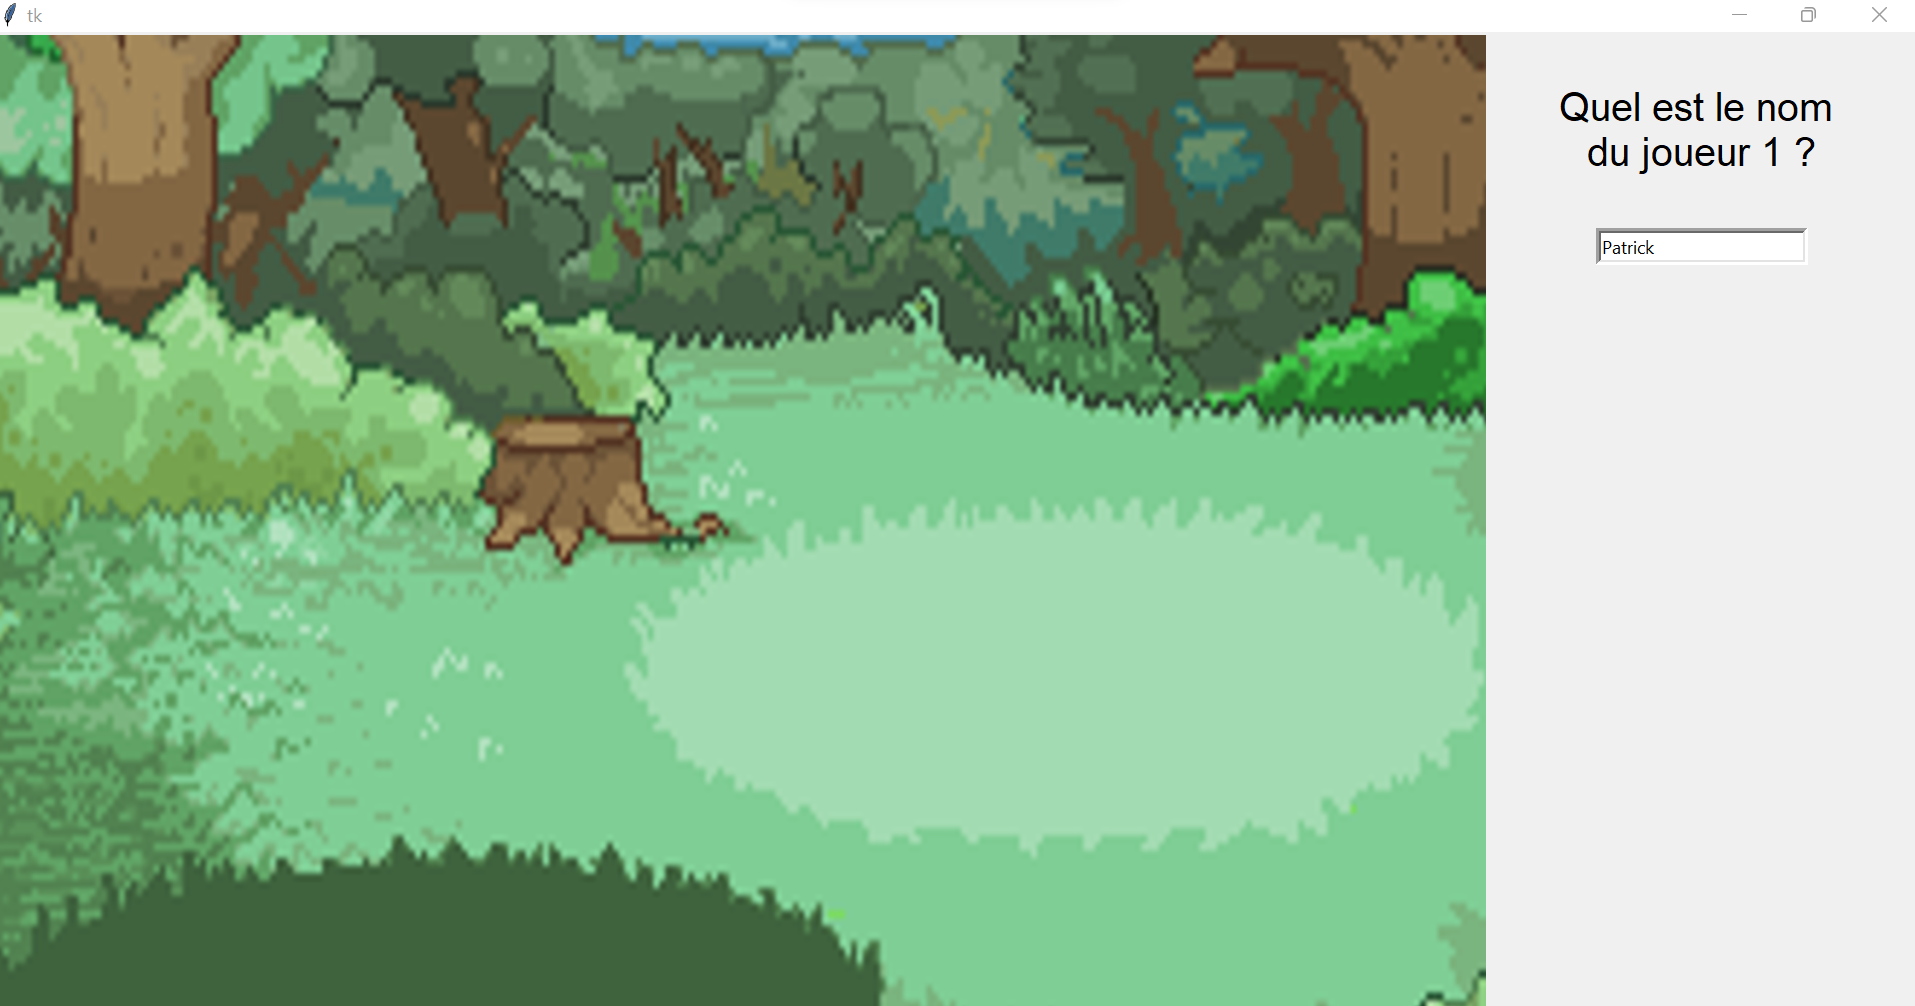
\includegraphics[width=13cm,height=7cm]{images/nom}
            
            Image 3: choix premier pokemon:
            
            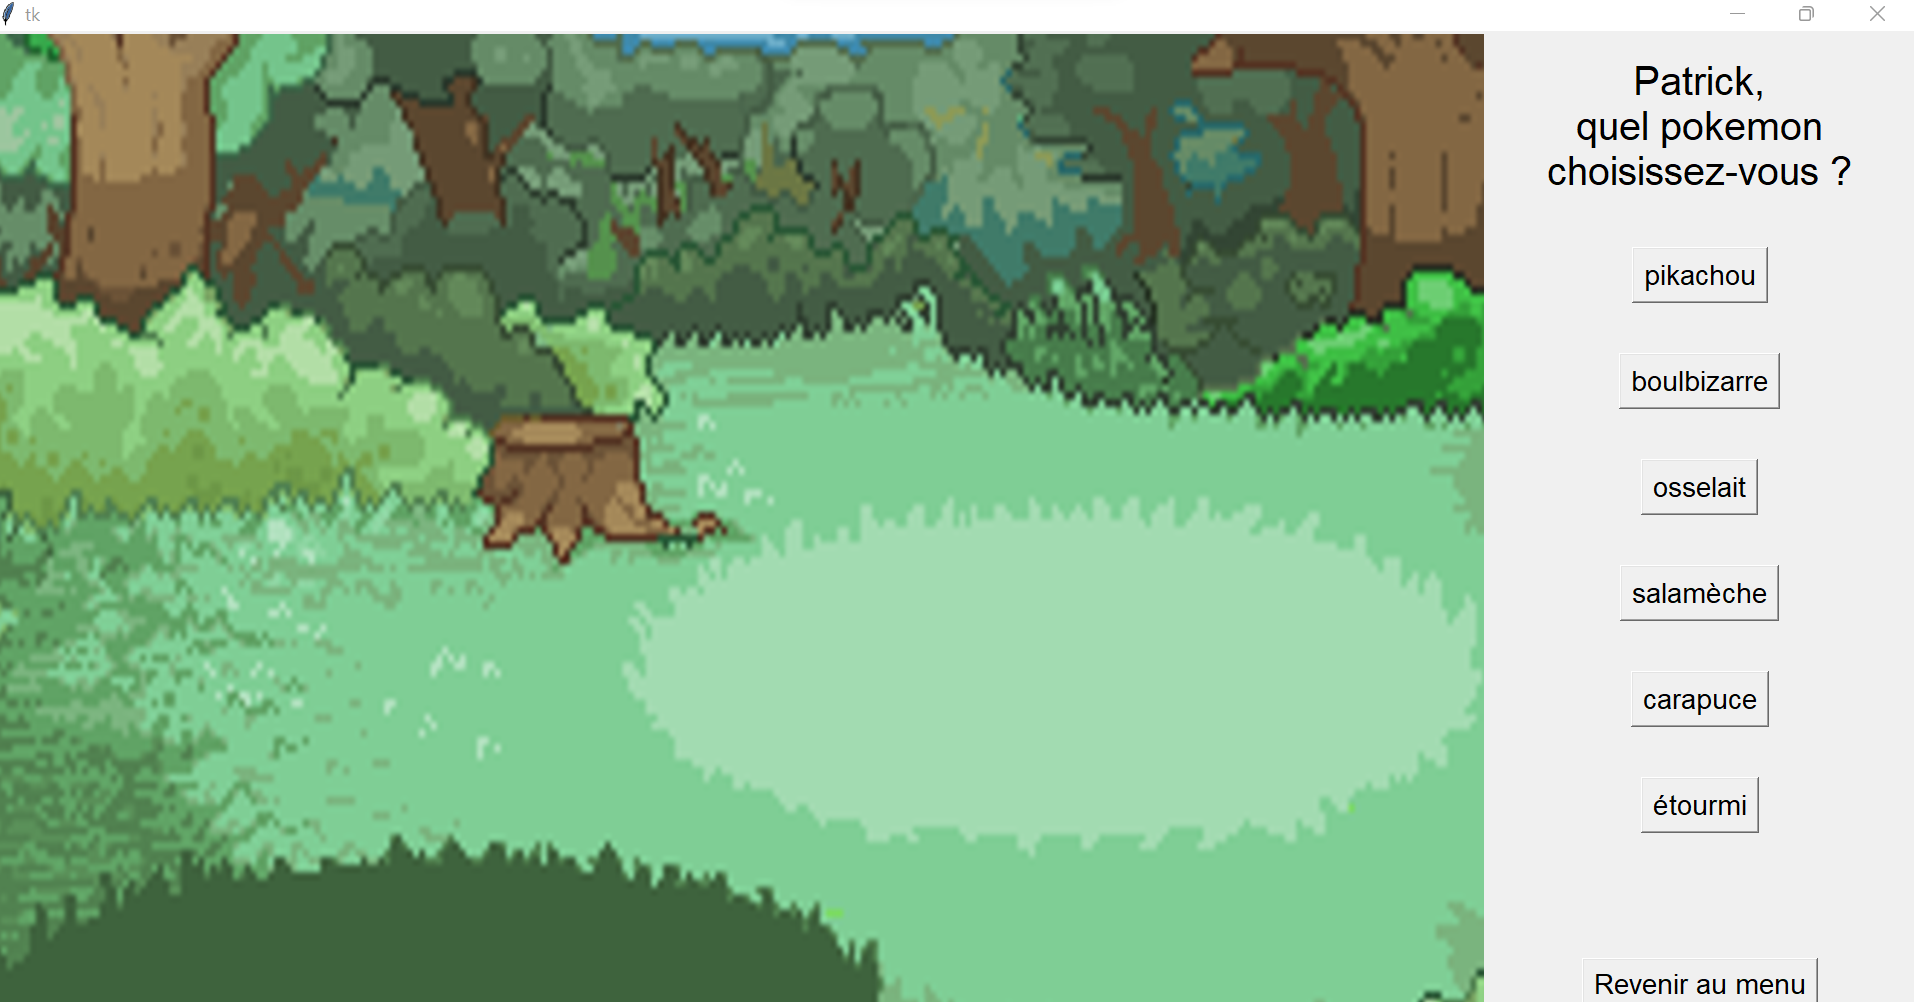
\includegraphics[width=13cm,height=7cm]{images/choix1}
            
            Image 4 : choix action :
            
            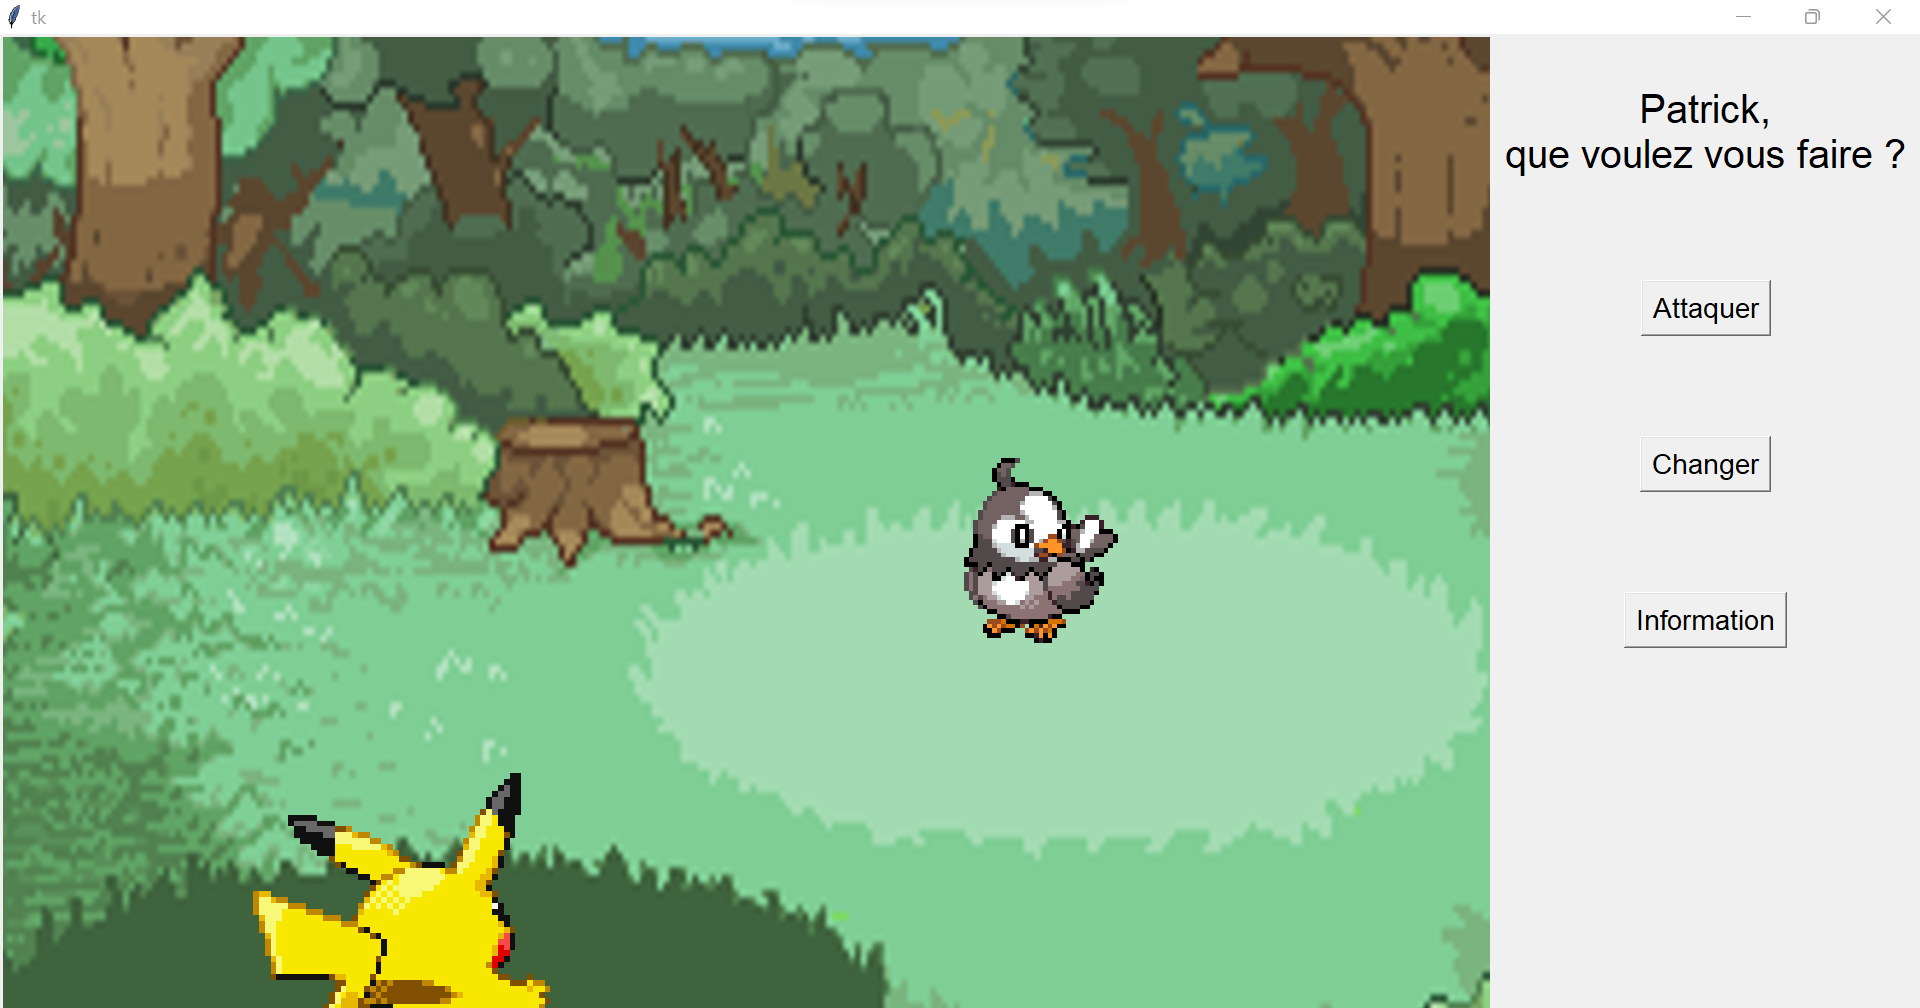
\includegraphics[width=13cm,height=7cm]{images/choix_action}
            
            Image 5 : choix des pokemons :
            
            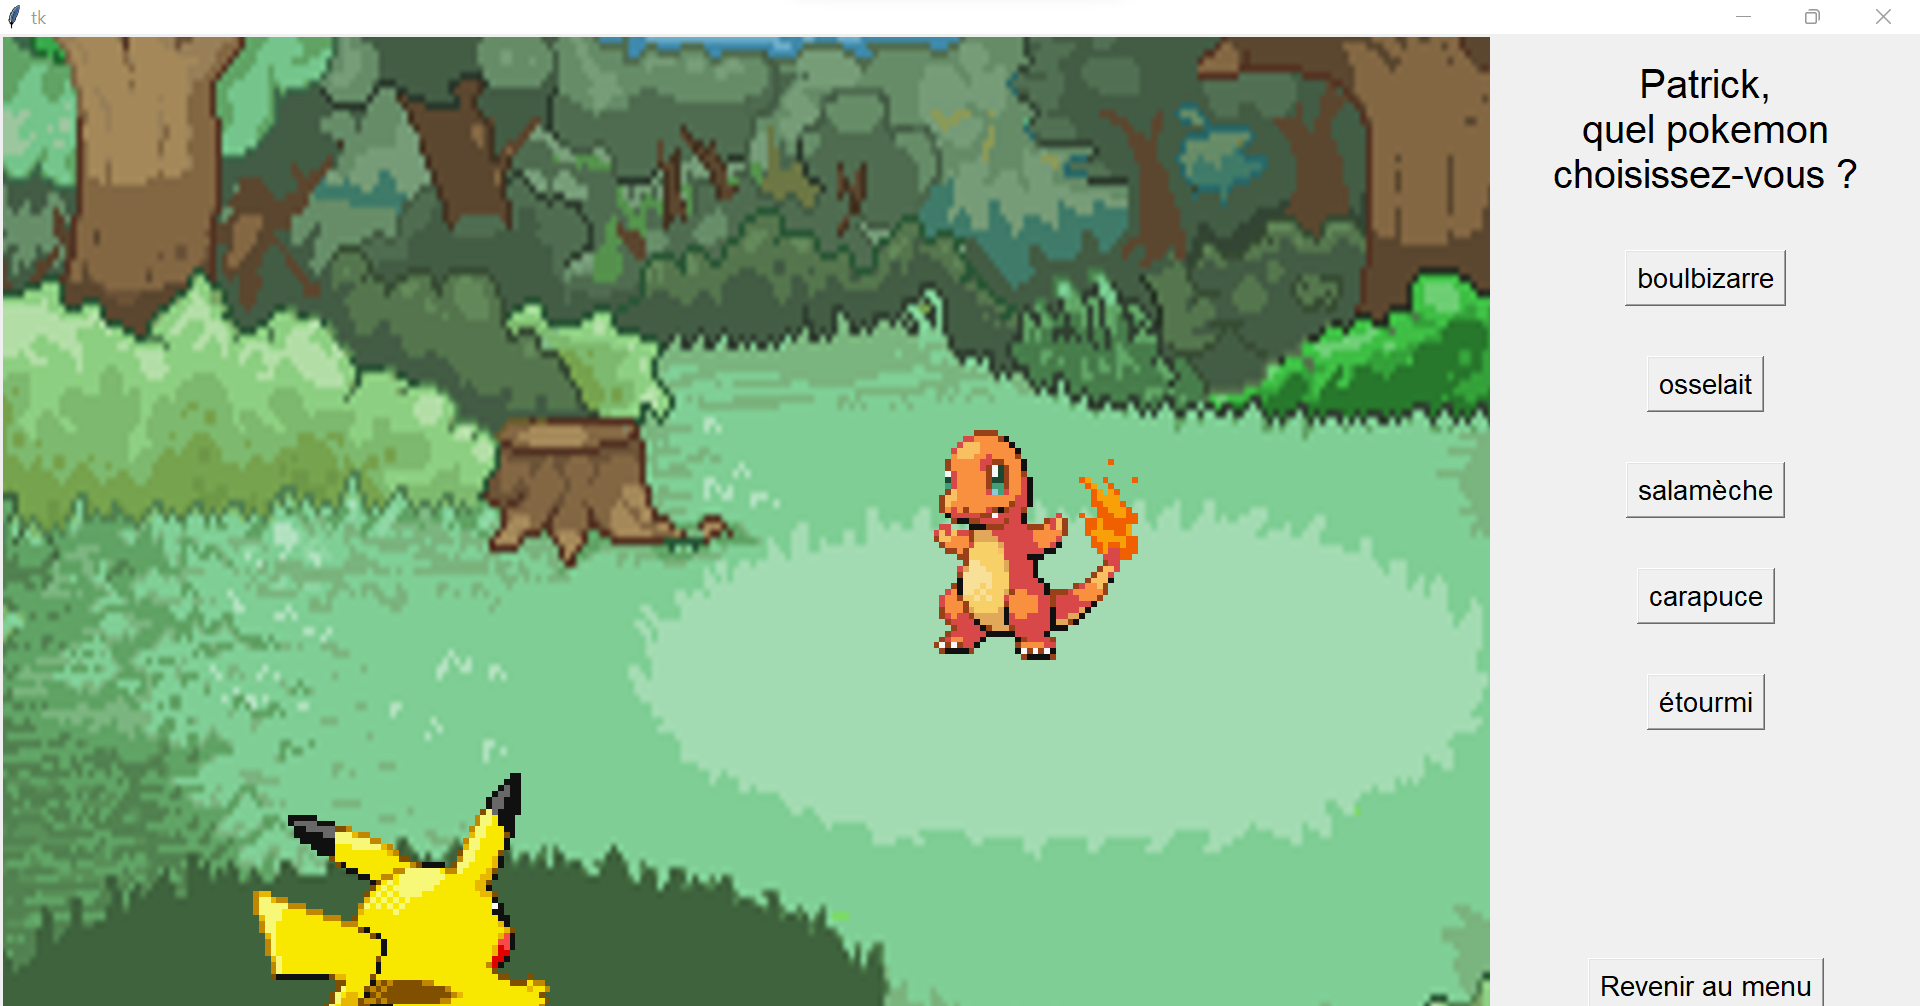
\includegraphics[width=13cm,height=7cm]{images/choix_poke}
            
            Image 6 : choix des attaques :
            
            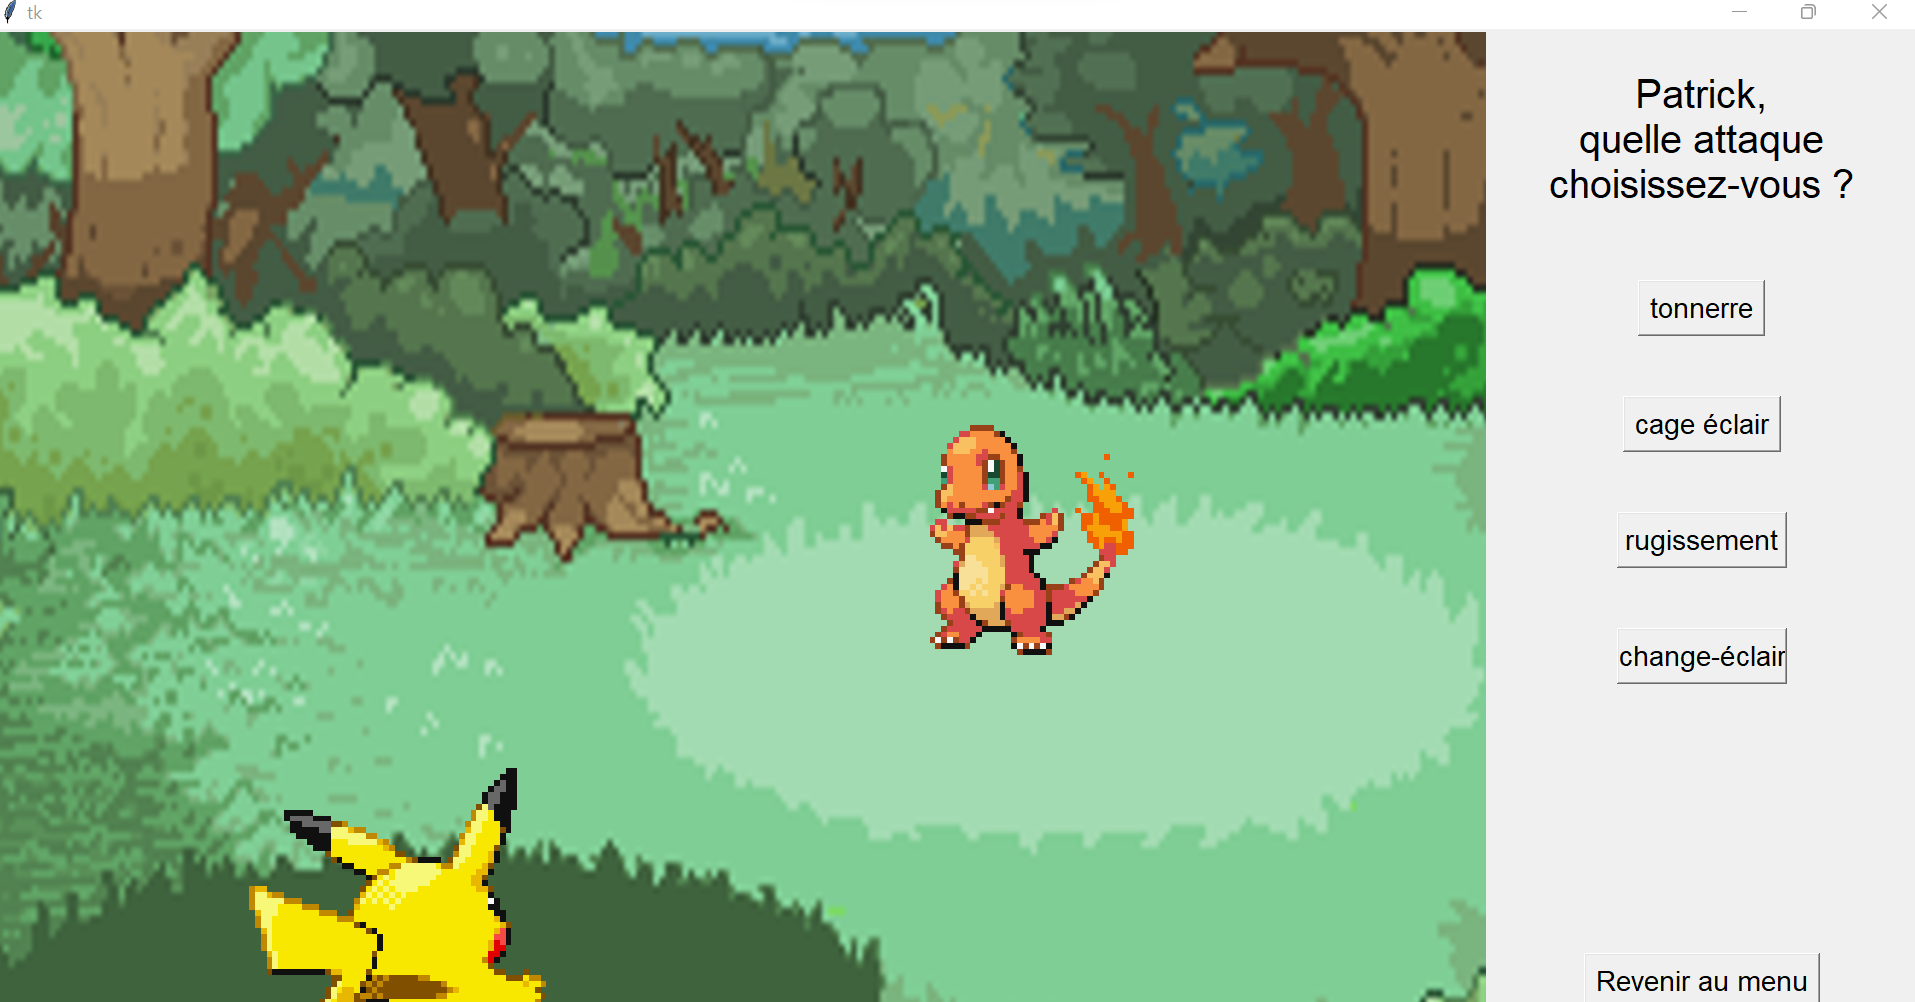
\includegraphics[width=13cm,height=7cm]{images/attaque}
            
            Images 7 : information:
            
            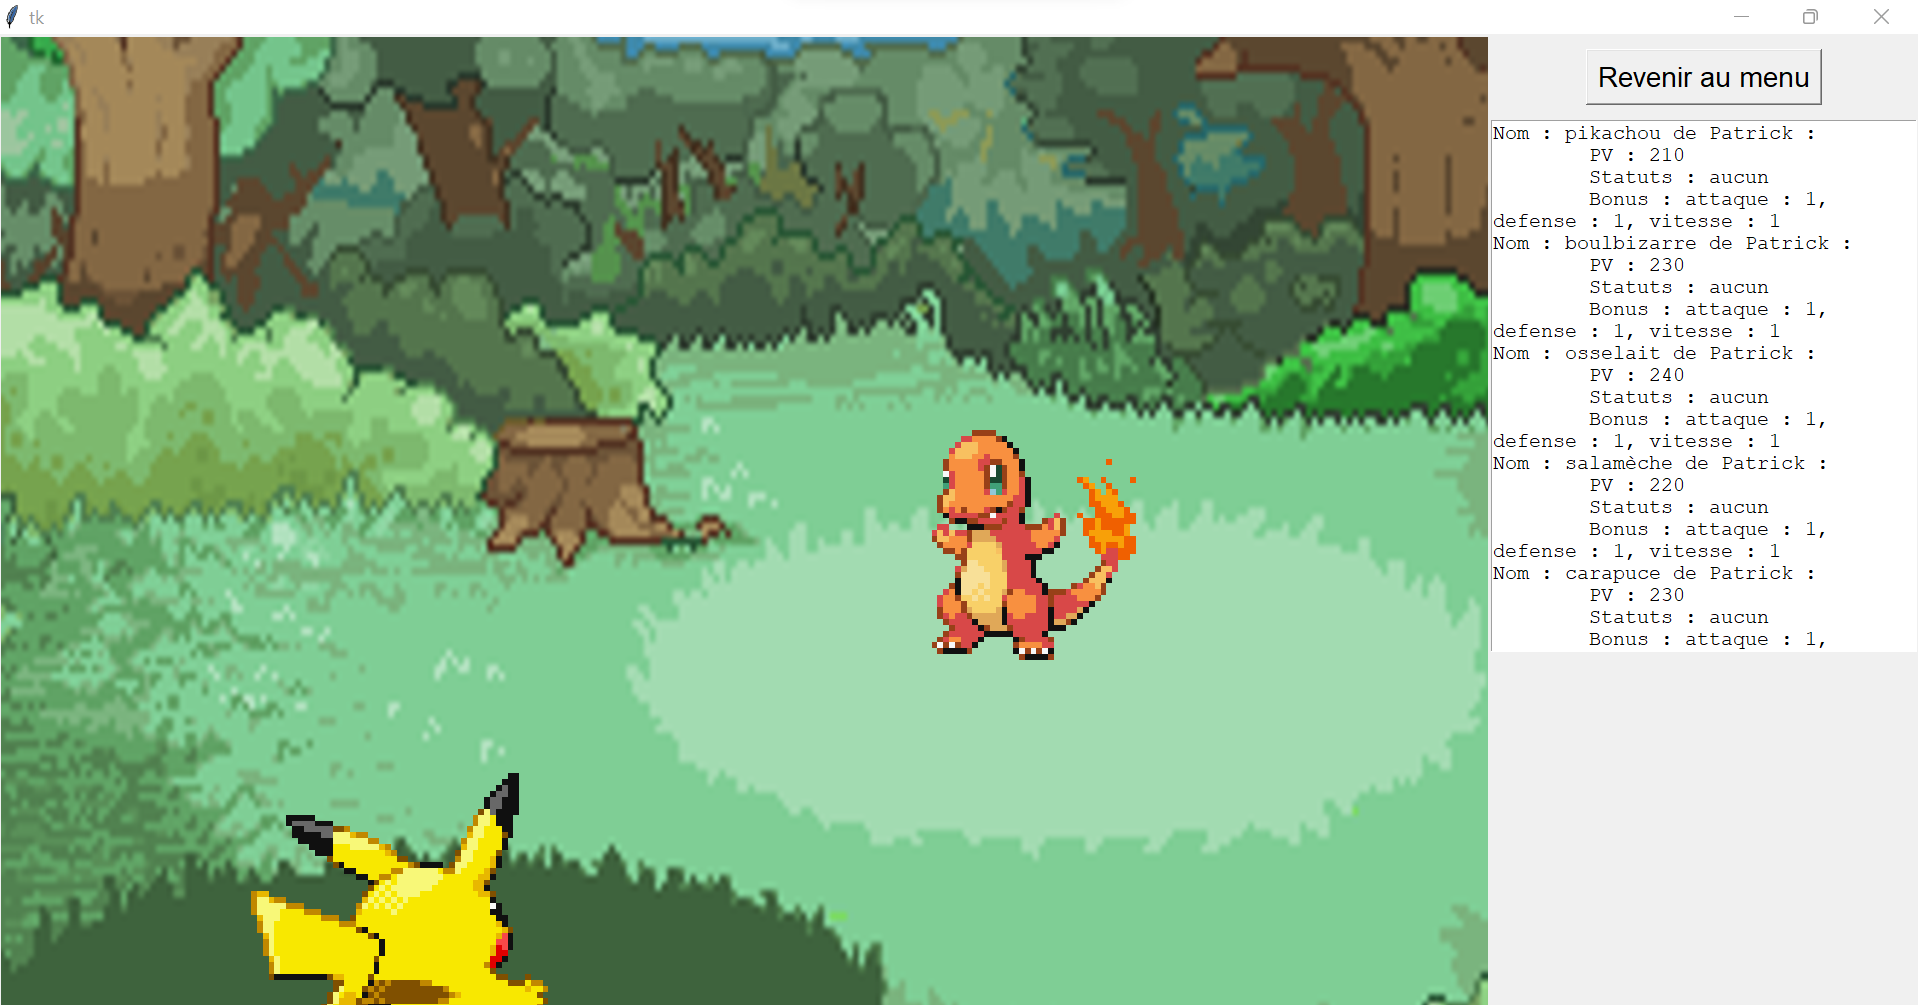
\includegraphics[width=13cm,height=7cm]{images/information}
            
            Images 8 : état du tour:
            
            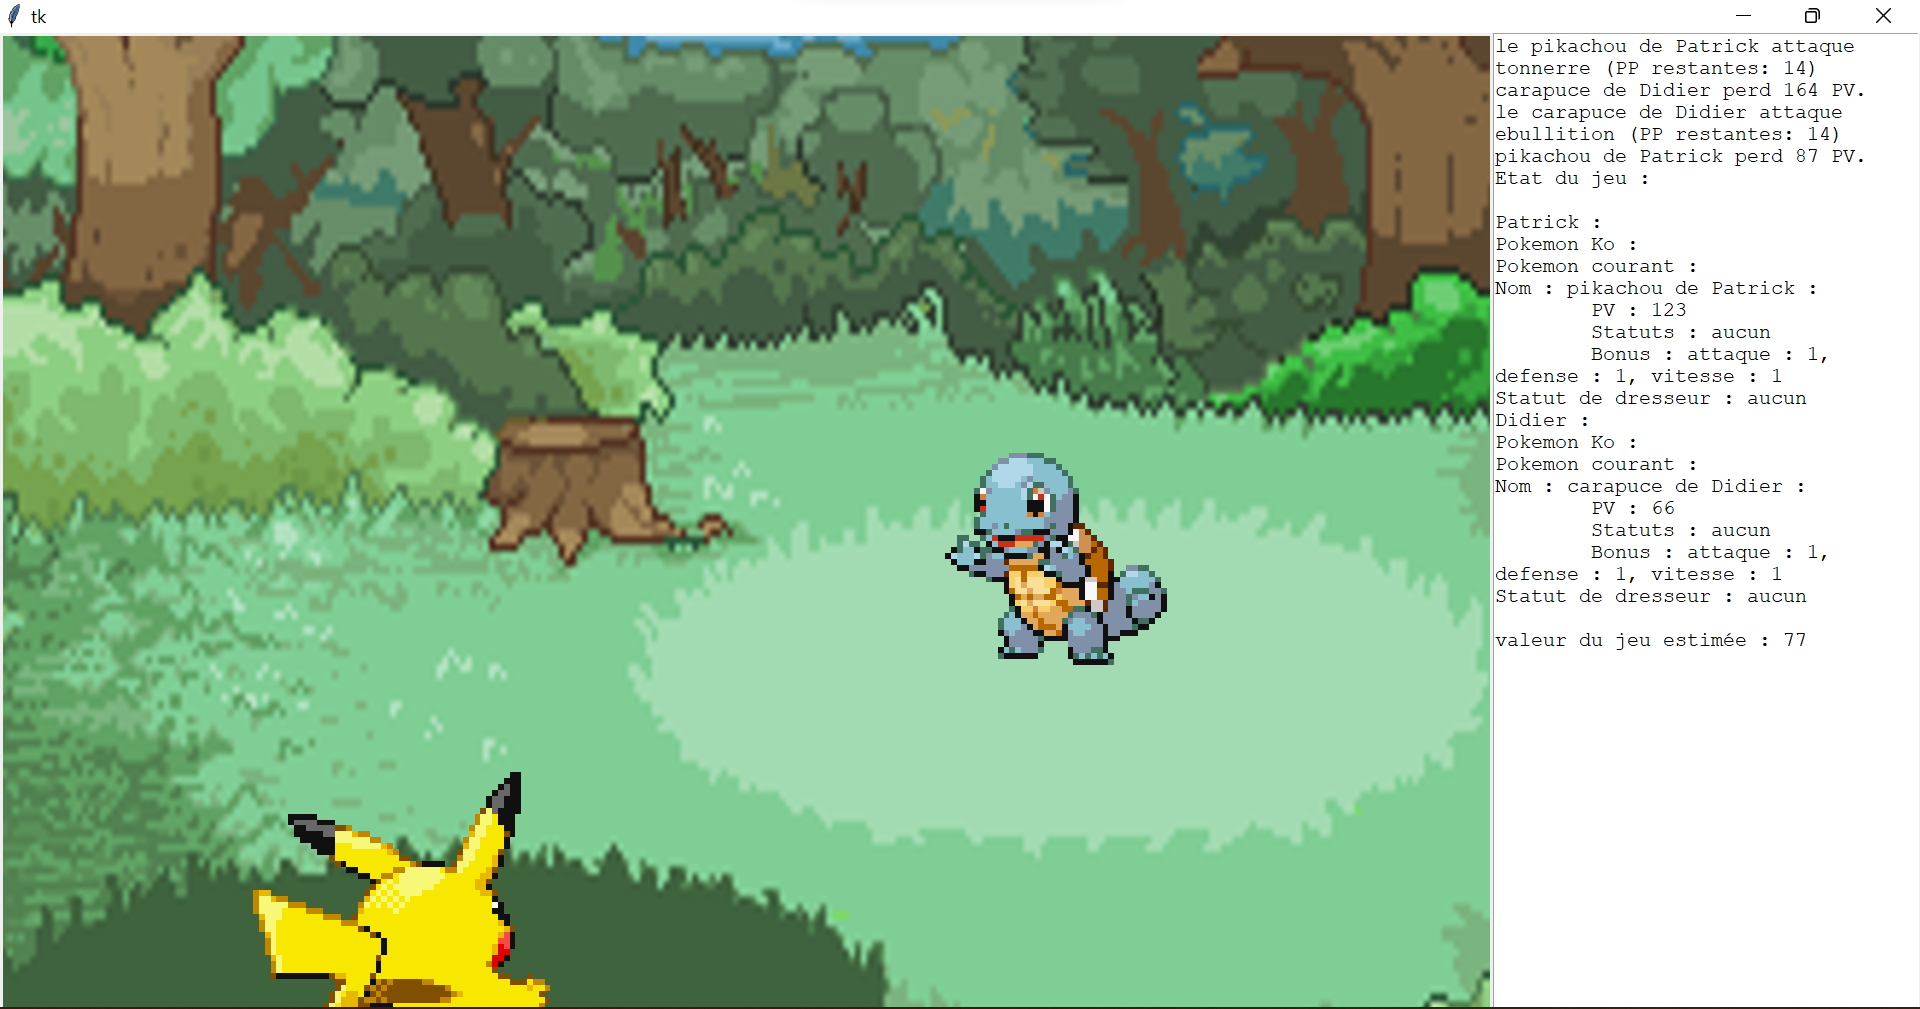
\includegraphics[width=13cm,height=7cm]{images/etat_tour}
            
            Images 9 : Fin de la partie:
            
            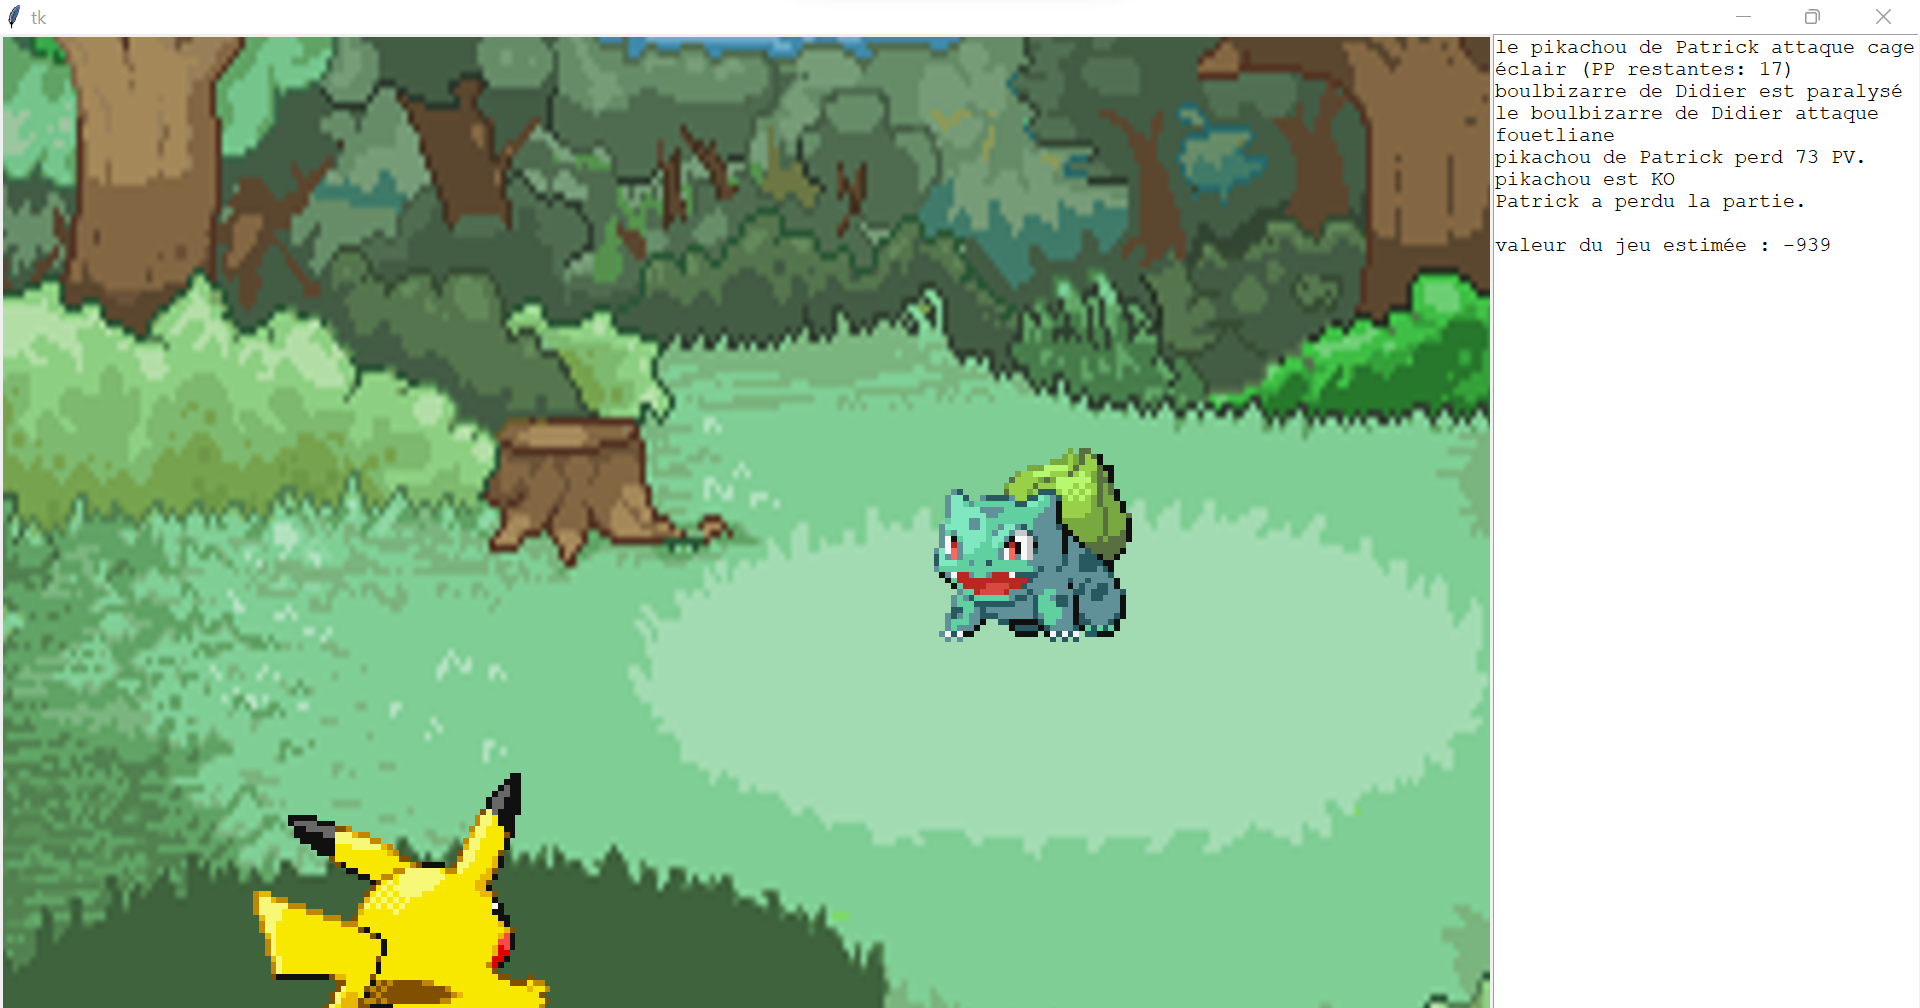
\includegraphics[width=13cm,height=7cm]{images/fin_partie}

            
        
    
        
        \section{Manuel utilisateur}
            Afin de pouvoir lancer le jeu, il est nécessaire de telecharger tout les fichiers fournis ainsi que les images, fournies également. Celles-ci sont à ranger dans un dossier 'images' pour la bonne éxecution du code. Une fois que tout est prêt, lancer le programme via le fichier 'main.py'. Une question portant sur le choix de l'interface vous sera alors posée. Une fois ce choix fait, la partie se lance. Suivez le déroulé des tours présenté dans les points 6.2.1 pour l'interface textuelle et 6.3.1 pour l'interface graphique. Ils détaillent les choix que vous serez amenés à faire ainsi que la méthode pour les donner, en plus d'indication pour pouvoir visualiser les différentes informations relatives à la partie en cours.
            
            Si vous voulez lancer un nombre important de partie, il faudra augment la profondeur maximale de récursion ligne 130 de abstract\_jeu.py
        \section{Sources}
    Le papier de recherche sur un ia deeplearning et pokemon : \textbf{Learning complex games through self play - Pokémon battles} de \emph{Miquel Llobet Sanchez} : https://upcommons.upc.edu/handle/2117/121655
    
    Des articles wikipédia qui nous ont été utiles :
    \begin{itemize}
		\item Minimax : https://en.wikipedia.org/wiki/Minimax
		\item Alpha Beta : https://en.wikipedia.org/wiki/Alpha%E2%80%93beta_pruning
		\item Expectiminimax : https://en.wikipedia.org/wiki/Expectiminimax
		\item PVS : https://en.wikipedia.org/wiki/Principal\_variation\_search
		\item Théorie des jeux : https://fr.wikipedia.org/wiki/Th%C3%A9orie_des_jeux
	\end{itemize}
   Pour toutes les informations/images concernant les pokemons: https://www.pokepedia.fr/Portail:Accueil et https://www.pokebip.com/
   (a noter que nos pokemons ont les noms des jeux réels mise à part Pikachou (Pikachu) et Boulbizarre (Bulbizarre)
   
   Un article sur l'ordre des mouvements : https://www.chessprogramming.org/Move\_Ordering
    
\end{document}
    
 